\documentclass[12pt,twoside]{article}

\newcommand{\reporttitle}{PalliCare}
\newcommand{\reportauthor}{Patrick H\"ofner, Klaus Schmidt, Ulla Sternemann, Insa Suchantke, Daniel Wagner}
\newcommand{\scrummaster}{Malte Ollenschl\"ager, Imrana Abdullahi Yari}
\newcommand{\projectpartner}{Dr. med. Tobias Steigleder, UK Erlangen}

% include files that load packages and define macros
%%%%%%%%%%%%%%%%%%%%%%%%%%%%%%%%%%%%%%%%%
% University Assignment Title Page 
% LaTeX Template
% Version 1.0 (27/12/12)
%
% This template has been downloaded from:
% http://www.LaTeXTemplates.com
%
% Original author:
% WikiBooks (http://en.wikibooks.org/wiki/LaTeX/Title_Creation)
%
% License:
% CC BY-NC-SA 3.0 (http://creativecommons.org/licenses/by-nc-sa/3.0/)
% 
% Instructions for using this template:
% This title page is capable of being compiled as is. This is not useful for 
% including it in another document. To do this, you have two options: 
%
% 1) Copy/paste everything between \begin{document} and \end{document} 
% starting at \begin{titlepage} and paste this into another LaTeX file where you 
% want your title page.
% OR
% 2) Remove everything outside the \begin{titlepage} and \end{titlepage} and 
% move this file to the same directory as the LaTeX file you wish to add it to. 
% Then add \input{./title_page_1.tex} to your LaTeX file where you want your
% title page.
%
%----------------------------------------------------------------------------------------
%	PACKAGES AND OTHER DOCUMENT CONFIGURATIONS
%----------------------------------------------------------------------------------------
\usepackage{ifxetex}
\usepackage{textpos}
\usepackage{natbib}
\usepackage{kpfonts}
\usepackage[a4paper,hmargin=2.8cm,vmargin=2.0cm,includeheadfoot]{geometry}
\usepackage{ifxetex}
\usepackage{stackengine}
\usepackage{tabularx,longtable,multirow,subfigure,caption}%hangcaption
\usepackage{fncylab} %formatting of labels
\usepackage{fancyhdr}
\usepackage{color}
\usepackage[tight,ugly]{units}
\usepackage{url}
\usepackage{float}
\usepackage[english]{babel}
\usepackage{amsmath}
\usepackage{graphicx}
\usepackage[colorinlistoftodos]{todonotes}
\usepackage{dsfont}
\usepackage{epstopdf} % automatically replace .eps with .pdf in graphics
\usepackage{natbib}
\usepackage{backref}
\usepackage{array}
\usepackage{latexsym}
\usepackage{etoolbox}

\usepackage{enumerate} % for numbering with [a)] format 

% additional usepackages
\usepackage{wrapfig}
\usepackage{listings}
%\usepackage[numbers]{natbib}
\setcitestyle{numbers}
\setcitestyle{square}
\setcitestyle{comma}


\ifxetex
\usepackage{fontspec}
\setmainfont[Scale=.8]{OpenDyslexic-Regular}
\else
\usepackage[pdftex,pagebackref,hypertexnames=false,colorlinks]{hyperref} % provide links in pdf
\hypersetup{pdftitle={},
  pdfsubject={}, 
  pdfauthor={\reportauthor},
  pdfkeywords={}, 
  pdfstartview=FitH,
  pdfpagemode={UseOutlines},% None, FullScreen, UseOutlines
  bookmarksnumbered=true, bookmarksopen=true, colorlinks,
    citecolor=black,%
    filecolor=black,%
    linkcolor=black,%
    urlcolor=black}
\usepackage[all]{hypcap}
\fi

\usepackage{tcolorbox}

% various theorems
\usepackage{ntheorem}
\theoremstyle{break}
\newtheorem{lemma}{Lemma}
\newtheorem{theorem}{Theorem}
\newtheorem{remark}{Remark}
\newtheorem{definition}{Definition}
\newtheorem{proof}{Proof}

% example-environment
\newenvironment{example}[1][]
{ 
\vspace{4mm}
\noindent\makebox[\linewidth]{\rule{\hsize}{1.5pt}}
\textbf{Example #1}\\
}
{ 
\noindent\newline\makebox[\linewidth]{\rule{\hsize}{1.0pt}}
}



%\renewcommand{\rmdefault}{pplx} % Palatino
% \renewcommand{\rmdefault}{put} % Utopia

\ifxetex
\else
\renewcommand*{\rmdefault}{bch} % Charter
\renewcommand*{\ttdefault}{cmtt} % Computer Modern Typewriter
%\renewcommand*{\rmdefault}{phv} % Helvetica
%\renewcommand*{\rmdefault}{iwona} % Avant Garde
\fi

\setlength{\parindent}{0em}  % indentation of paragraph

\setlength{\headheight}{14.5pt}
\pagestyle{fancy}
\fancyfoot[ER,OL]{\thepage}%Page no. in the left on
                                %odd pages and on right on even pages
\fancyfoot[OC,EC]{\sffamily }
\renewcommand{\headrulewidth}{0.1pt}
\renewcommand{\footrulewidth}{0.1pt}
\captionsetup{margin=10pt,font=small,labelfont=bf}


%--- chapter heading

\def\@makechapterhead#1{%
  \vspace*{10\p@}%
  {\parindent \z@ \raggedright %\sffamily
        %{\Large \MakeUppercase{\@chapapp} \space \thechapter}
        %\\
        %\hrulefill
        %\par\nobreak
        %\vskip 10\p@
    \interlinepenalty\@M
    \Huge \bfseries 
    \thechapter \space\space #1\par\nobreak
    \vskip 30\p@
  }}

%---chapter heading for \chapter*  
\def\@makeschapterhead#1{%
  \vspace*{10\p@}%
  {\parindent \z@ \raggedright
    \sffamily
    \interlinepenalty\@M
    \Huge \bfseries  
    #1\par\nobreak
    \vskip 30\p@
  }}
  



% %%%%%%%%%%%%% boxit
\def\Beginboxit
   {\par
    \vbox\bgroup
	   \hrule
	   \hbox\bgroup
		  \vrule \kern1.2pt %
		  \vbox\bgroup\kern1.2pt
   }

\def\Endboxit{%
			      \kern1.2pt
		       \egroup
		  \kern1.2pt\vrule
		\egroup
	   \hrule
	 \egroup
   }	

\newenvironment{boxit}{\Beginboxit}{\Endboxit}
\newenvironment{boxit*}{\Beginboxit\hbox to\hsize{}}{\Endboxit}



\allowdisplaybreaks

\makeatletter
\newcounter{elimination@steps}
\newcolumntype{R}[1]{>{\raggedleft\arraybackslash$}p{#1}<{$}}
\def\elimination@num@rights{}
\def\elimination@num@variables{}
\def\elimination@col@width{}
\newenvironment{elimination}[4][0]
{
    \setcounter{elimination@steps}{0}
    \def\elimination@num@rights{#1}
    \def\elimination@num@variables{#2}
    \def\elimination@col@width{#3}
    \renewcommand{\arraystretch}{#4}
    \start@align\@ne\st@rredtrue\m@ne
}
{
    \endalign
    \ignorespacesafterend
}
\newcommand{\eliminationstep}[2]
{
    \ifnum\value{elimination@steps}>0\leadsto\quad\fi
    \left[
        \ifnum\elimination@num@rights>0
            \begin{array}
            {@{}*{\elimination@num@variables}{R{\elimination@col@width}}
            |@{}*{\elimination@num@rights}{R{\elimination@col@width}}}
        \else
            \begin{array}
            {@{}*{\elimination@num@variables}{R{\elimination@col@width}}}
        \fi
            #1
        \end{array}
    \right]
    & 
    \begin{array}{l}
        #2
    \end{array}
    &%                                    moved second & here
    \addtocounter{elimination@steps}{1}
}
\makeatother

%% Fast macro for column vectors
\makeatletter  
\def\colvec#1{\expandafter\colvec@i#1,,,,,,,,,\@nil}
\def\colvec@i#1,#2,#3,#4,#5,#6,#7,#8,#9\@nil{% 
  \ifx$#2$ \begin{bmatrix}#1\end{bmatrix} \else
    \ifx$#3$ \begin{bmatrix}#1\\#2\end{bmatrix} \else
      \ifx$#4$ \begin{bmatrix}#1\\#2\\#3\end{bmatrix}\else
        \ifx$#5$ \begin{bmatrix}#1\\#2\\#3\\#4\end{bmatrix}\else
          \ifx$#6$ \begin{bmatrix}#1\\#2\\#3\\#4\\#5\end{bmatrix}\else
            \ifx$#7$ \begin{bmatrix}#1\\#2\\#3\\#4\\#5\\#6\end{bmatrix}\else
              \ifx$#8$ \begin{bmatrix}#1\\#2\\#3\\#4\\#5\\#6\\#7\end{bmatrix}\else
                 \PackageError{Column Vector}{The vector you tried to write is too big, use bmatrix instead}{Try using the bmatrix environment}
              \fi
            \fi
          \fi
        \fi
      \fi
    \fi
  \fi 
}  
\makeatother

\robustify{\colvec}

%%% Local Variables: 
%%% mode: latex
%%% TeX-master: "notes"
%%% End: 
 % various packages needed for maths etc.

%%%%%%%%%%%%%%%%%%%%%%%%%%%%

\begin{document}
% front page
% Last modification: 2016-09-29 (Marc Deisenroth)
\begin{titlepage}

\newcommand{\HRule}{\rule{\linewidth}{0.5mm}} % Defines a new command for the horizontal lines, change thickness here


%----------------------------------------------------------------------------------------
%	LOGO SECTION
%----------------------------------------------------------------------------------------


\includegraphics[width = 6cm]{./figures/FAU_logo} 
\hspace{3cm}

\includegraphics[width = 6cm]{./figures/FAU_logo}\\[0.5cm] 

\begin{center} % Center remainder of the page

%----------------------------------------------------------------------------------------
%	HEADING SECTIONS
%----------------------------------------------------------------------------------------
\textsc{\LARGE Innovation Lab for Wearable and Ubiquitous Computing}\\[1 cm] 
\textsc{\Large Machine Learning and Data Analytics Lab}\\[0.5cm] 
\textsc{\large Department of Computer Science}\\[0.5cm] 
%----------------------------------------------------------------------------------------
%	TITLE SECTION
%----------------------------------------------------------------------------------------

\HRule \\[0.4cm]
{ \huge \bfseries \reporttitle}\\ % Title of your document
\HRule \\[1.5cm]
\end{center}
%----------------------------------------------------------------------------------------
%	AUTHOR SECTION
%----------------------------------------------------------------------------------------

%\begin{minipage}{0.4\hsize}
\begin{flushleft} \large
\textit{Students:}\\
\reportauthor \\% Your name
\vspace{1cm}
\textit{Project partner:}
\projectpartner\\ % partners name
\vspace{1cm}
\textit{Scrum master:} \\ % Your supervisor
\scrummaster
\end{flushleft}
\vspace{1cm}
\makeatletter
Date: \@date 

\vfill % Fill the rest of the page with whitespace



\makeatother


\end{titlepage}



%%%%%%%%%%%%%%%%%%%%%%%%%%%% Main document
\section{Introduction}
\subsection{Definition of Palliative Care}
Palliative care is the treatment, accompaniment and care of seriously ill and dying people \cite{rki1}. More than half of the palliative patients suffer from cancer, 29.2 \% suffer from a disease of the circulatory system, 5.6 \% from a neurological and 0.3 \% from other underlying diseases \cite{pruetz}. The aim of palliative care is to improve the quality of the remaining life of such patients and their families by preventing and alleviating the disease through early detection, assessment and treatment of pain and psychological, spiritual and psychosocial problems \cite{radbruch}.  
\newline  In Germany, approximately 90 \% of the nearly 850,000 deaths per year require palliative care \cite{radbruch}. The 326 specialized ambulatory palliative care (SAPC) teams and more than 330 palliative stations and units, which exist in Germany, need support to be able to fulfill the wish of 76 \% of Germans to die at home \cite{hospiz, grote}. Unfortunately only 20 \% of Germans die at home. Almost 46 \% die in hospitals, 31 \% in old people's homes and 3 \% in hospices \cite{grote}.
\newline Obviously, many more people want to stay and could also die at home if there would be sufficient capacity of care services. It is therefore necessary to develop a product that supports the SAPC teams and gives the patient the opportunity to die at home or to be cared for at home for as long as possible.  

\subsection{Project explanation}
This project has developed a product called \textit{PalliCare}. For this product an android smartphone application (app) for the patient and a web interface for the SAPC teams has been developed.  
The smartphone app which has been developed in Java has been designed for two user groups, on the one hand for palliative patients and on the other hand for their closest relatives, also called next of kin (nok). The app records and displays the biometric (body weight, blood pressure) and psychometric data (a minimal documentation system called MIDOS questionnaire \cite{midos}) for the palliative patients. Body weight is measured with a body scale which is connected with the app via Bluetooth connection. The blood pressure and the MIDOS questionnaire have to be entered manually. In addition, the patient can store emergency contacts, to whom she/he can contact via an emergency button if she/he is not feeling well. 
In the nok mode of the app, the relatives can view the recorded data of the patient, if it has been authorized by the patient beforehand.
The web interface is intended for the SAPC teams to view the health status of their patients. The data of the patients is shown and listed by priority.

\section{Insa Suchantke}
\textbf{Responsibility: App development, Design decisions}\\
\textbf{Role: Organisation Master}\\

\subsection{Available smartphone apps in palliative care}
There are not many smartphone apps for palliative care on the market \cite{nwosu}. One of these apps is \textit{Alberta}\footnote{https://halloalberta.de} which is a care management platform for chronically ill patients to manage the entire patient care digitally. It has various features like digital documentation, appointment and route planning and complete patient files with all patient-related data. Another app is \textit{PalliDoc}\footnote{https://www.pallidoc.de} which is a software for palliative care. It offers for example team-specific overviews, task management, care documentation, symptom recording and determination of travel routes.
With the \textit{biotronik}\footnote{https://www.biotronik.com/en-de/patients/patientapp} app the cardiac status of patients with an implanted BIOTRONIK cardiac monitor BIOMONITOR III can be measured. In this app there also exists a diary function of the symptoms. \textit{Myo}\footnote{https://myo.de} app is a platform for communication between caregivers and relatives. The app \textit{vivifyhealth}\footnote{https://www.vivifyhealth.com} offers a remote patient monitoring platform for chronic and post-acute care with for example informative content for the patients and monitoring the biometric data of the patient.

Furthermore, there are also smartphone apps that provide information and facts about palliative care, such as \textit{Palliative Care Fast Facts}, \textit{Pocketbook of Palliative Medicine}, \textit{NHS Palliative Care Guidelines} and \textit{Palliative Care ACT}.

The Alberta and PalliDoc apps are the only ones that offer patient management. Only \textit{biotronics} and \textit{vivifyhealth} provide an integration of medical devices. \textit{PalliDoc}, \textit{myo} and \textit{vivifyhealth} have an interface for the care team and the doctor. An interface also for nok is just available at \textit{myo}. The apps \textit{biotronik} and \textit{vivifyhealth} make it possible to monitor the patients' state of health. 

Although all these apps provide nice features like patient management, integration of medical devices, interfaces for doctor, care teams or nok and monitoring the patients‘ state of health, no app combines the shared accessibility for patient, nok and SAPC team with data analysis and health status monitoring of the patient. Such an interdisciplinary platform must exist so that patients can be cared for at home and be enabled to die with care.

\subsection{PalliCare Smarthpone App - Design and layout decisions}
Most of the palliative patients have ages between 70 and 79 years with an average age of 70 \cite{rki1}. Because of that the layout of the \textit{PalliCare} smartphone app had to be adapted to the high average age of these patients. In order to get a feeling what kind of layout and design is appropriate for older people, it has been examined which apps are already on the market for this age category.   

One of these apps is the \textit{SwissVoice CS50s}\footnote{https://www.swissvoice.net/de/produkt/c50s-0} smartphone, which has adapted features and layout for older people. For example, the ringtone and volume can be adjusted to an extra loud level and has further large icons to aid comprehensibility. The smartphone app \textit{Koala Phone Launcher Free}\footnote{https://tomas-slavicek-koala-phone.de.aptoide.com} is intended for older people who use the smartphone for the first time and also for those who have an visual impairment. The keyboard is kept large and the text is easy to read, as well as notifications are displayed in a clearly visible way. The \textit{Medisafe Alarm}\footnote{https://apps.apple.com/de/app/arznei-medikamente-alarm/id573916946} app supports the user in taking medication also with a reminder alarm. The layout is kept simple with a good contrast and a clear menu. The texts are kept short and easy to understand. To train the brain, the app \textit{Lumosity}\footnote{https://www.lumosity.com/} offers exercises. The menu is also kept clear, simple and understandable by so-called card layouts. There are also explanations for the individual exercises \cite{zabel}.   
\newline \newline The important features of the \textit{PalliCare} smartphone app, derived from the apps that are available on the market for older people, are listed below: 
\begin{itemize}
\item Simple menu
\item Consistent layout 
\item Large icons, buttons and font
\item Simple reminder function
\item Explanations
\end{itemize}

The \textit{PalliCare} app has a simple menu with a card layout for better overview, readability and comprehensibility of the menu. The colours and the contrast of the card layout were chosen to allow easy visibility of the contents of the app pages. The buttons and the font on each app page have been kept as big as possible for easy understanding. This is intended to simplify the selection of the buttons and makes it easier to read for patients with impaired vision. Icons were integrated to support the understanding of the button function. Therefore the layout was kept simple and understandable. The size of the card layouts, the buttons, the texts and the icons were kept uniform to support the comprehensibility of the app and to avoid confusion on the part of the layout. 
Furthermore, there is a help button on every page of the app which explains in short and with concise sentences about the respective function of the current active app page. This is intended to support the patient not feeling of being overwhelmed arises and that the patient does not feel lost. 
\newline In summary, \textit{PalliCare}  has a design and layout adapted to the mostly older palliative patients. It offers patient management, health status monitoring, medical device integration, an interface for care teams, doctors and nok and an analysis of the collected health data of the patients. This makes the \textit{PalliCare} app unique on the market.

\subsection{Welcome and Permission screens}
To gain the trust, trustworthiness and acceptance of the user, a welcome screen appears the first time the app is opened. The text is short, concise and contains all important information. It describes the function of the app without explicitly specifying how to use the app. Furthermore, the user should still have the feeling that everything is under her/his control. Therefore, it must be explained exactly what the app is for, what data is recorded and informs about the data privacy. Furthermore, no unnecessary distraction should be created and the colours and logos should be kept uniform \cite{just, liquide}. 

There are two different texts, depending on whether the user is a palliative patient or a nok. The text for the palliative patient informs about the data recording and the emergency button (see Figure \ref{fig:welcome_patient}).  
\newline \newline
\fbox{\parbox{\textwidth}{„Willkommen bei PalliCare! Ich werde dir dabei helfen, deine Gesundheitsdaten aufzuzeichnen. Ich erfasse deine Gesundheitsdaten, damit ich dir Informationen über deine Gesundheit geben kann. Du bekommst einen sofortigen Überblick über deine gemessenen Werte und deinen Gesundheitszustand. Auch kann ich im Notfall, falls es dir nicht gut gehen sollte, deine Familie kontaktieren. Durch dich kann ich auch anderen Menschen, die in einer ähnlichen Situation wie du sind, helfen. Ich kann deine gesammelten Daten zur Vorhersage des Gesundheitszustandes dieser Menschen nutzen. Lass uns beginnen!“}}
\newline
\begin{figure}[H]
    \centering
    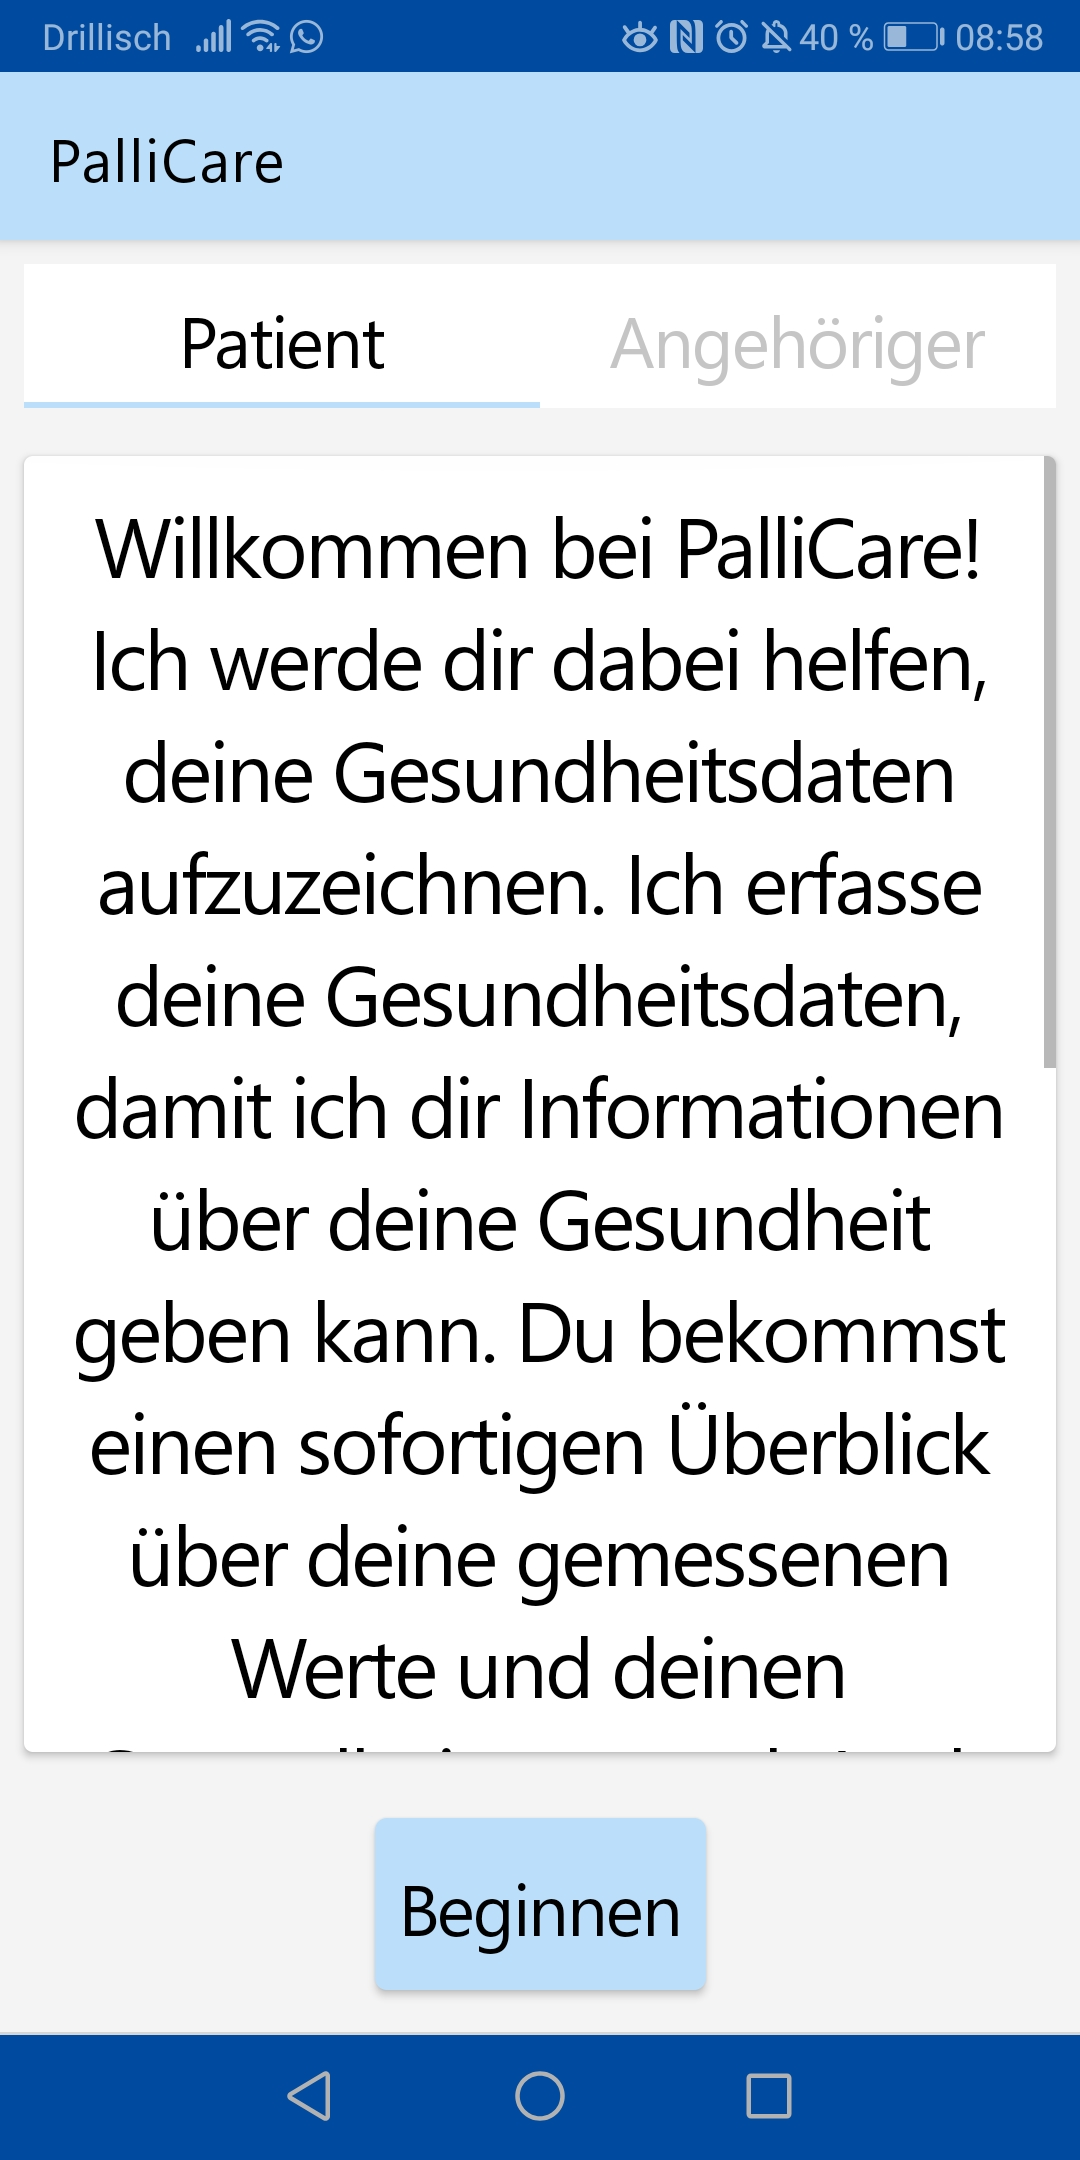
\includegraphics[width=4cm]{figures/welcome_patient.png}
    \caption{Welcome Screen for palliative patients}
    \label{fig:welcome_patient}
\end{figure}
The welcome text for the nok contains the information that the user is a contact and emergency person and that the user has an overview of the patient's data (see Figure \ref{fig:welcome_nok}). 
\newline \newline
\fbox{\parbox{\textwidth}{„Willkommen bei PalliCare! Sie werden eine Kontakt- und Notfallperson für einen Patienten sein. Ich werde die Gesundheitsdaten des Patienten aufzeichnen, damit ich ihm/ihr Informationen über die Gesundheit geben kann. Sie können diese Daten anschauen und somit einen Überblick über den Gesundheitszustand des Patienten bekommen. Im Notfall, falls es dem Patienten nicht gut geht, werden Sie benachrichtigt und somit sofort eingreifen, falls es ihm/ihr nicht gut gehen sollte. Durch Sie wird sich der Patient sicher fühlen und auch Sie werden immer einen Überblick über den Gesundheitszustand des Patienten haben. Lass uns beginnen!“}}
\begin{figure}[H]
    \centering
    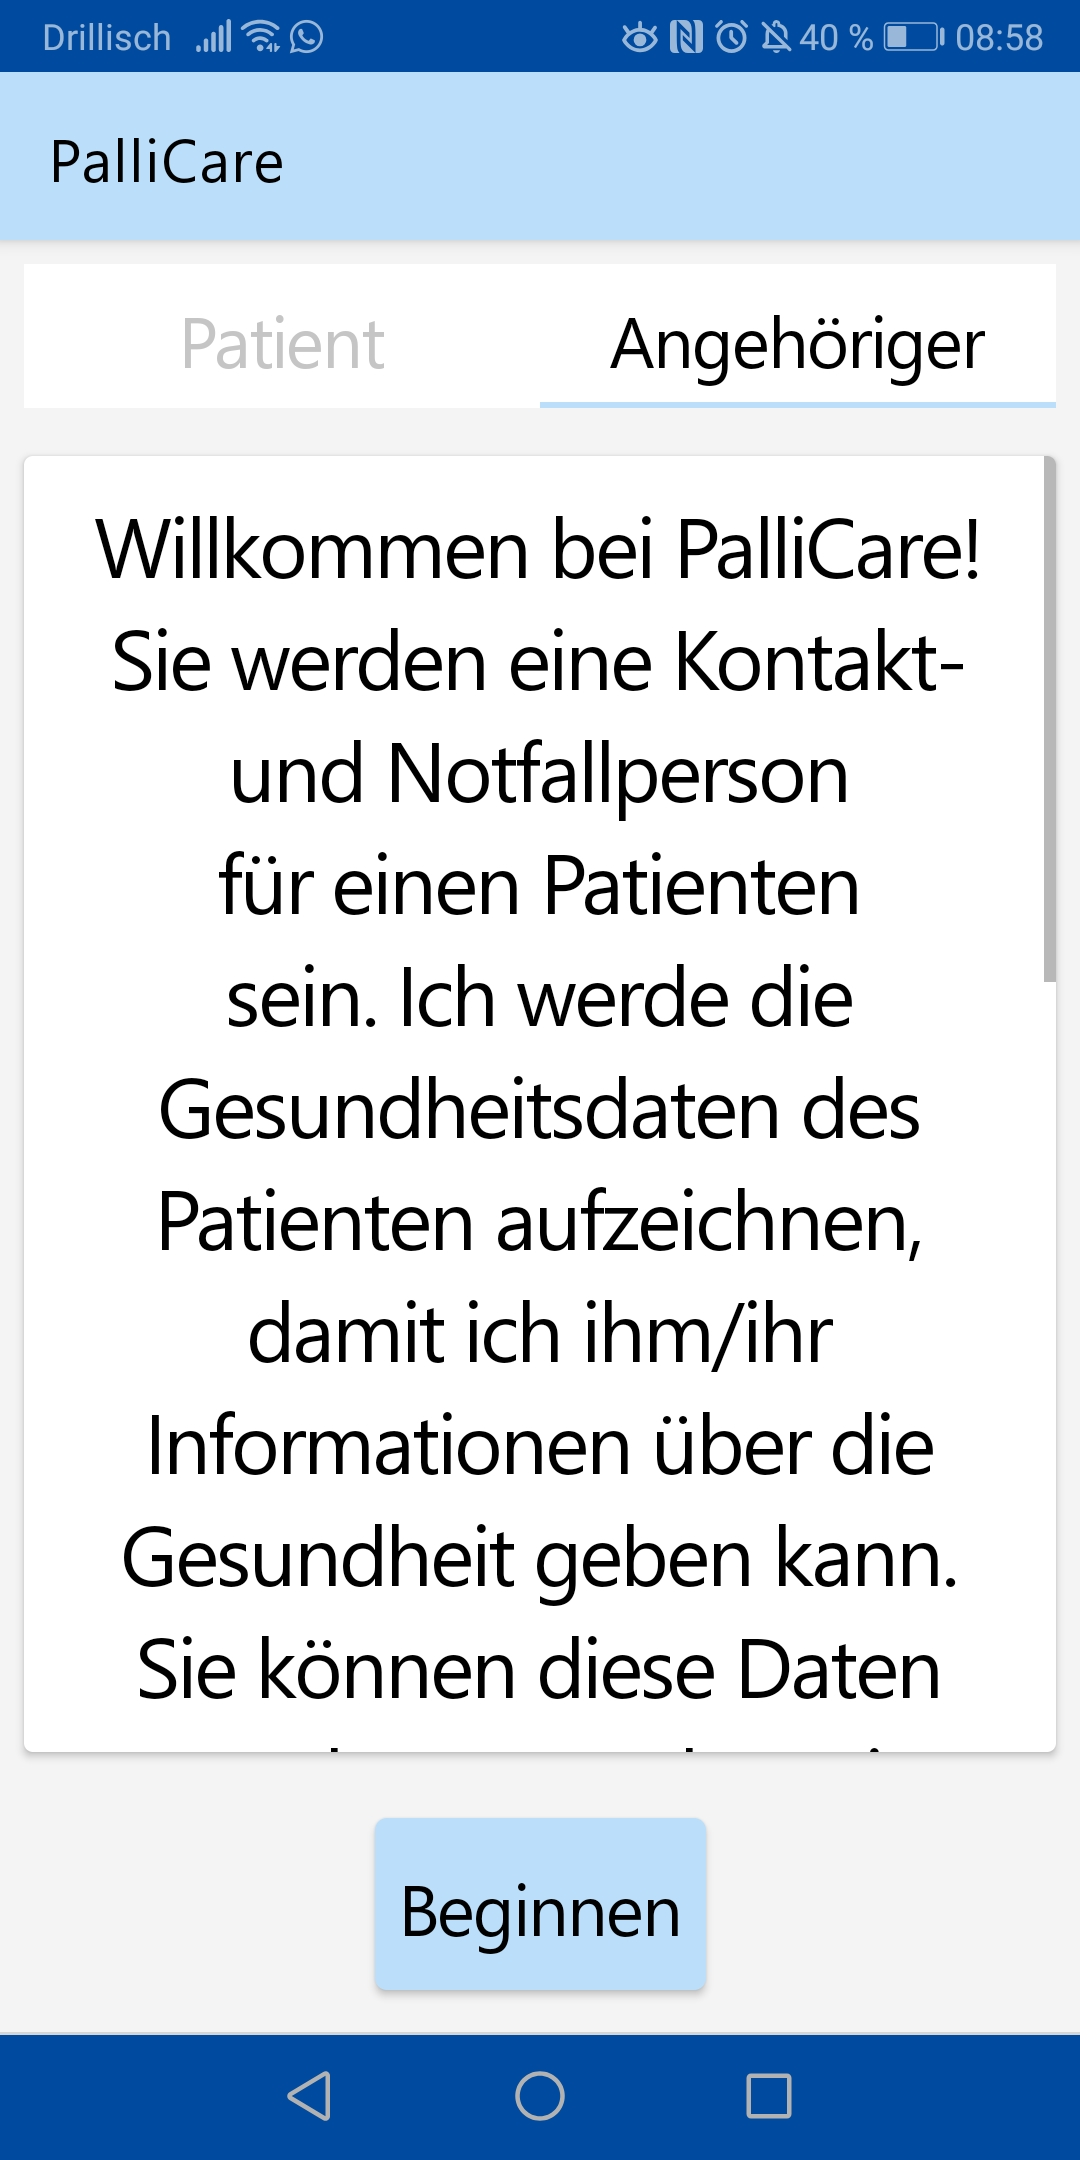
\includegraphics[width=4cm]{figures/welcome_nok.jpg}
    \caption{Welcome Screen for nok}
    \label{fig:welcome_nok}
\end{figure}
After the welcome screen the user has to accept some permissions that are needed for the use of the app. 

First the user must accept the bluetooth permission. This is needed to allow the app to connect to the body scale to record the body weight. This connection also requires access to the location.
\newline \newline
\fbox{\parbox{\textwidth}{„Zur Erfassung Ihrer Gesundheitsdaten wird die Waage mit Ihrem Smartphone über Bluetooth verbunden. Dafür wird der Zugriff auf Ihren Standort benötigt, damit die Verbindung funktionieren kann.“}}
\newline \newline
Afterwards the permission for external and internal storage is required so that the patient's data can be stored on the smartphone.
\newline \newline
\fbox{\parbox{\textwidth}{„Die App erfasst auch Ihre Gesundheitsdaten, damit sie Ihnen Informationen über Ihre Gesundheit geben kann. Zur Speicherung Ihrer Daten benötigen wir Ihre Erlaubnis, dass diese Daten auf Ihrem Handyspeicher gespeichert werden können.“}}
\newline \newline
The last permission is for the emergency button so that the app can make a call. If a patient uses the emergency button, one of the stored emergency contacts is automatically called. 
\newline \newline
\fbox{\parbox{\textwidth}{„Im Folgenden benötigt die App einige Zugriffsberechtigungen. Falls es Ihnen nicht gut gehen sollte, können Sie im Notfall mit Hilfe der App eine Person anrufen, deren Nummer Sie vorher eingespeichert haben. Dafür benötigt die App Ihre Erlaubnis, jemanden anzurufen. Die App verwendet nicht Ihr Telefonbuch.“}}

\section{Klaus-Günther Schmidt}
\textbf{Responsibility: Android development, Bluetooth synchronization, MIDOS integration}\\
\textbf{Role: Git Master}\\

As mentioned earlier, the average palliative patient is about 70 years old. Enabling them to stay in homecare by using a mobile app with connected sensors, is a big advantage as well as a challenge.

Usually, older people are not used to interact with latest technology and due to suffering from serious diseases they often have limited mental and physical capabilities.

To deal with this problem, we decided to make the usage of our app as simple as possible. In order to support this with our implementation we focused on a simple, intuitive as well as consistent design and structure of our app.

\subsection{Prototyping with Adobe XD}
To prevent troubles when starting the actual implementation with Android Studio\footnote{https://developer.android.com/studio}, we decided to construct a mockup of our app. Therefore, I created a set of app activities, which were tested and reviewed by the other team members. This led to valuable feedback such that we were able to improve the app even before we had written a single line of code. 

We decided to create a horizontal and high fidelity prototype. The horizontal aspect means that we implement a broad overview of the app without specific, in-depth functionality. Thus, we were able to get a general overview of what the app should and might include. Furthermore, it allowed us to add or remove features with ease, not spending too much time in making things look beautiful and to ultimately identify mandatory and optional parts of our product.

A high fidelity prototype offers a realistic look and feel. This enabled us to discuss the design, layout, colors with focus on the typical capabilities and age of a palliative care patient.

To build such a mockup, we decided to use Adobe XD\footnote{https://www.adobe.com/de/products/xd.html}. It is a free-to-use tool, which has an extensive yet simple interface builder. It supports drag-and-drop to add and rearrange different shapes, text boxes, images, etc. It is possible to define common UI elements, colors as well as fonts. It even allows to model connections between the different activities so that one receives an interactive prototype.

This led to our first implementation (see Figure \ref{fig:xd}), which allowed us to continue with the planning:

 At first, we split up the app in multiple parts: Login/Registration, Homescreen, Emergency, Settings, acquiring and display of biometrical and physiometrical health information, next of kin and doctor interface. Thus, we were able to prioritize the different features. For example the acquisition and display of information as well as the emergency screen were mandatory features, while the settings and the next of kin interface were less important considering the aims of the project. Therefore, we decided to remove the doctors' interface from the Android app completely.
 
Grouping the different activities also allowed us to assign different people to the different packages so that we could implement them independently from each other.
Furthermore, we talked about the general activity design (see Chapter \ref{chap:baseactivity}) and came up with several ideas of how to keep the interface easy to understand and clean for the patients.

\begin{figure}[]
\vspace{-10pt}
    \centering
    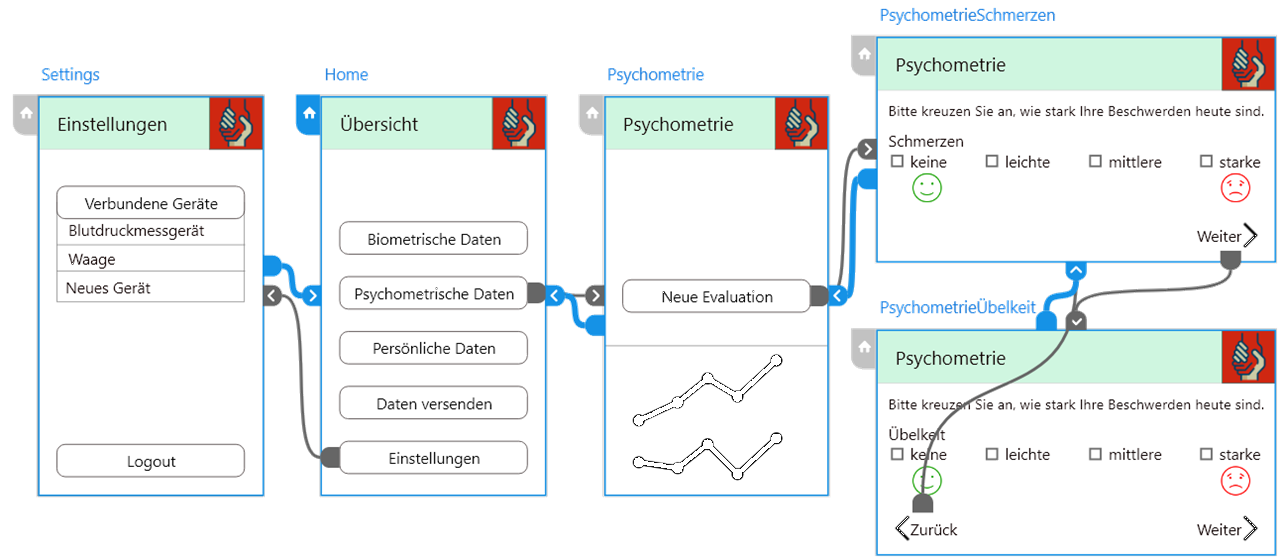
\includegraphics[width=\textwidth]{figures/KlausXD.png}
    \caption{Part of the prototype with activity connections - Screenshot AdobeXD}
    \label{fig:xd}
\end{figure}

\subsection{Defining a general app layout}
\label{chap:baseactivity}
At first, each developer started to use his own design and screen layout. By doing very similar work multiple times we were able to identify different implementation approaches for the common elements. Apart from that, we peer reviewed the different implementations. Therefore, we collected many ideas that we considered as very important.
My job was to combine all those identified aspects to be eventually able to have a common activity design as well as functionality.

Therefore, I implemented a BaseActivity class, which defines the primary visual structure of our app, featuring a help button which provides an explanation for each screen, and an emergency button to call help from any screen with only two touches.

\subsubsection{BaseActivitys}
The BaseActivity class is an abstract class which is the superclass of all of the activities for a registered user. The main purpose of the BaseActivity is to define the visual structure of these inheriting activities. This means, each activity inheriting from the BaseActivity, has the predefined main layout, but is still able to show custom text and components (see Figure \ref{fig:baseactivity}). A big advantage of this is that a future change of the common layout does not have to be done in each activity manually. Instead, it is just necessary to change the BaseActivity.

\begin{wrapfigure}{r}{0.32\textwidth}
\vspace{-10pt}
  \begin{center}
    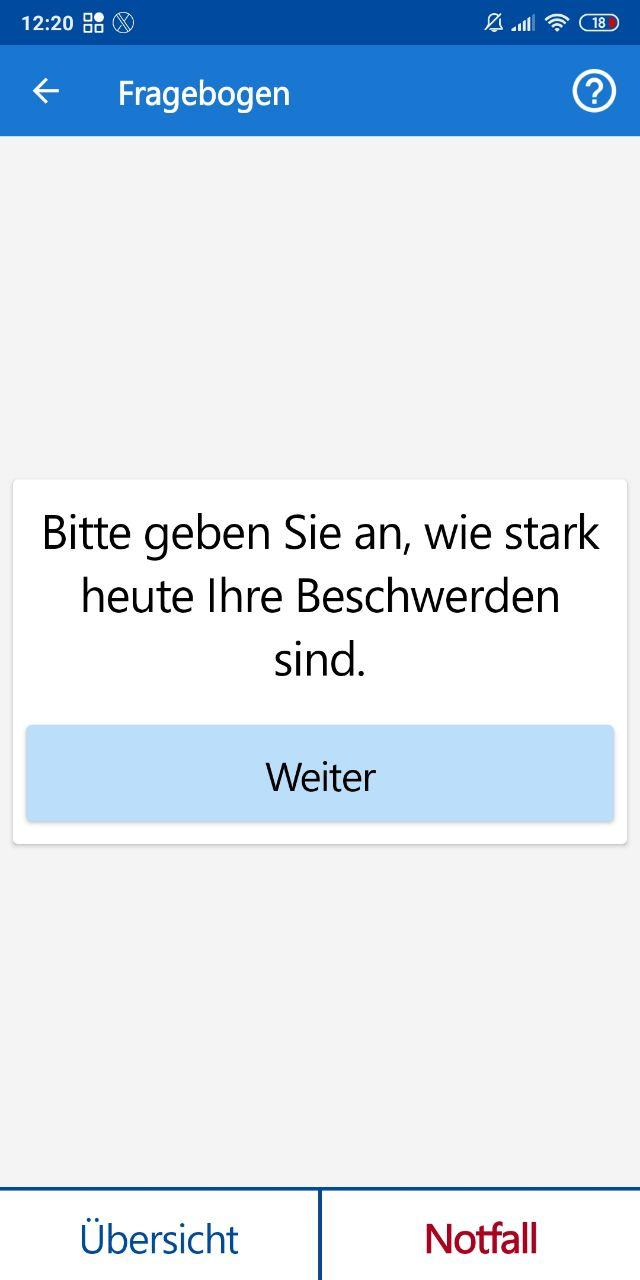
\includegraphics[width=0.30\textwidth]{figures/KlausBasicActivity.jpg}
  \end{center}
  \caption{Implementation of the BaseActivity}
  \label{fig:baseactivity}
  \vspace{-30pt}
\end{wrapfigure}
At the top of any activity, which extends the BaseActivity, is an ActionBar. The ActionBar itself is splitted into three parts: an optional back-button to access the prior activity, the title of the current activity and the help button.

For each inheriting activity it is possible to hide the back button, when it does not make sense, to change the activity title
    and to change the text which is displayed after clicking the help button.
    
At the bottom of any activity extending the BaseActivity there is a panel with two buttons: the first to return to the home screen and the second to reach the emergency activity. These buttons are very important for the patients. The home button enables them to return to the default overview screen to prevent them from being lost in the app. The emergency button enables a patient to call for help (e.g. ambulance, doctor or a next of kin) within just two clicks. 
It is possible to disable each button separately. For example in the emergency screen itself, it is not necessary to show the emergency button (see Figure \ref{fig:emergency}).

\subsubsection{Emergency Screen}
\begin{wrapfigure}{r}{0.32\textwidth}
\vspace{-30pt}
\begin{center}
    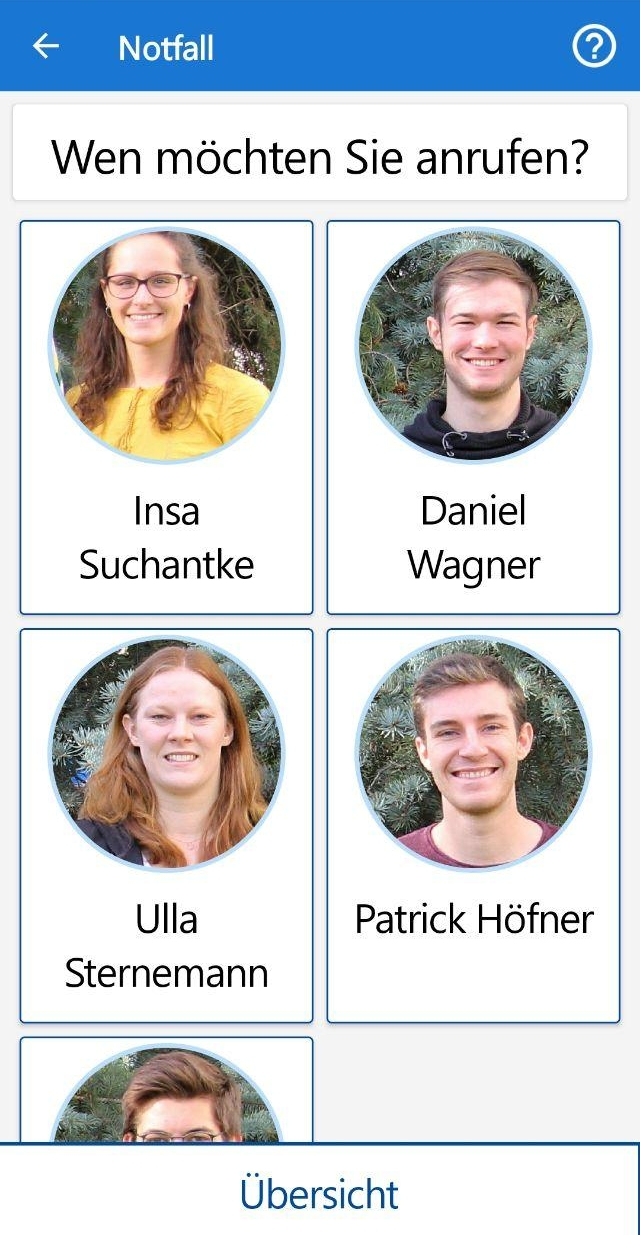
\includegraphics[width=0.30\textwidth]{figures/KlausEmergency.jpg}
  \end{center}
  \caption{Emergency Screen with Contacts}
  \label{fig:emergency}
  \vspace{-30pt}
\end{wrapfigure}
The emergency screen is a very simple to use and essential feature in our app. It enables a patient to call preassigned emergency contacts when feeling sick or suffering from exceptional pain. Each contact card consists of a (not visible) number, the name and an optional contact picture. When clicking on a contact card, the defined number is called immediately. This is realized by a simple Intent of the type ACTION\_CALL.

It was important to us that this emergency call feature is accessible in a quick way. That is why we included it in the already mentioned BaseActivity.

To be able to show the round contact images, we use the CircleImageView library\footnote{https://github.com/hdodenhof/CircleImageView} from Henning Dodenhof. It is licensed under Apache License, Version 2.0.

In the current prototype it is not possible for a patient to add custom contacts. So far only the contacts of our team are hardcoded into the app. For the following studies, the functionality will be improved to allow to add and call custom emergency contacts. Furthermore, it is planned, after clarifying the legal aspects, to include the German emergency telephone number 112 into the app as a hardcoded default "contact".

\subsubsection{Help Text}
\begin{wrapfigure}{r}{0.30\textwidth}
\vspace{-30pt}
  \begin{center}
    
\includegraphics[width=0.30\textwidth]{figures/KlausHelpText.jpg}
  \end{center}
  \caption{Examplary help text}
  \label{fig:helptext}
  \vspace{-10pt}
\end{wrapfigure}
To provide guidance for every activity, we decided to implement the help text feature. By clicking at the questionmark button in the upper right corner (see Figure \ref{fig:baseactivity}) a new dialog is opened (see Figure \ref{fig:helptext}). The shown text can be customized per activity by overriding the abstract method getHelpText() from the BaseActivity (see Listing \ref{lst:helptext}).
 
Theoretically, there would have been an oneliner solution to set the help text by defining a string variable, which is used by the BaseActivity. However, this may result in developers forgetting to set the help text correctly. Instead, by defining the text through the implementation of the abstract method, the creator of an activity is enforced to overwrite this getHelpText() method. I have, therefore, opted for this implementation to support the developers by reminding them to set this helptext.
\begin{lstlisting}[language=Java, label={lst:helptext}, caption={Implementation of the getHelpText method in the emergency activity},captionpos=b]
    @Override
    protected int getHelpText() {
        return R.string.help_emergency;
    }
\end{lstlisting}

\subsection{MIDOS questionnaire}
The MIDOS questionnaire \cite{midos} is a brief and simple survey for the self examination of the condition of a palliative patient. It is used by several institutions, including the palliative care department of the Universitätsklinikum Erlangen. By collecting daily information of the patient, e.g. pain, nausea, anxiety or lack of appetite, it is possible to get an idea of the physical and psychological state of the patient. These aspects are very important, as palliative care deals with the "treatment of pain and other problems, physical, psychosocial and spiritual.", as defined by the World Health Organization\footnote{https://www.who.int/cancer/palliative/definition/en/}.

MIDOS consists of multiple single choice questions (up to 5 answer options) and 3 free text questions. My goal was to keep the digitized version of the questionnaire as easy and similar to filling it out with pen and paper.

The first step was to break the survey down into small parts which can be shown at the screen in a good readable font size so that the patient is not overstrained. This resulted in showing just one task at a time and a next / previous button which let the user go one step for- or backward (see Figure \ref{fig:midos1}).

\begin{wrapfigure}{r}{0.35\textwidth}
\vspace{-10pt}
  \begin{center}
  %TODO correct picture
    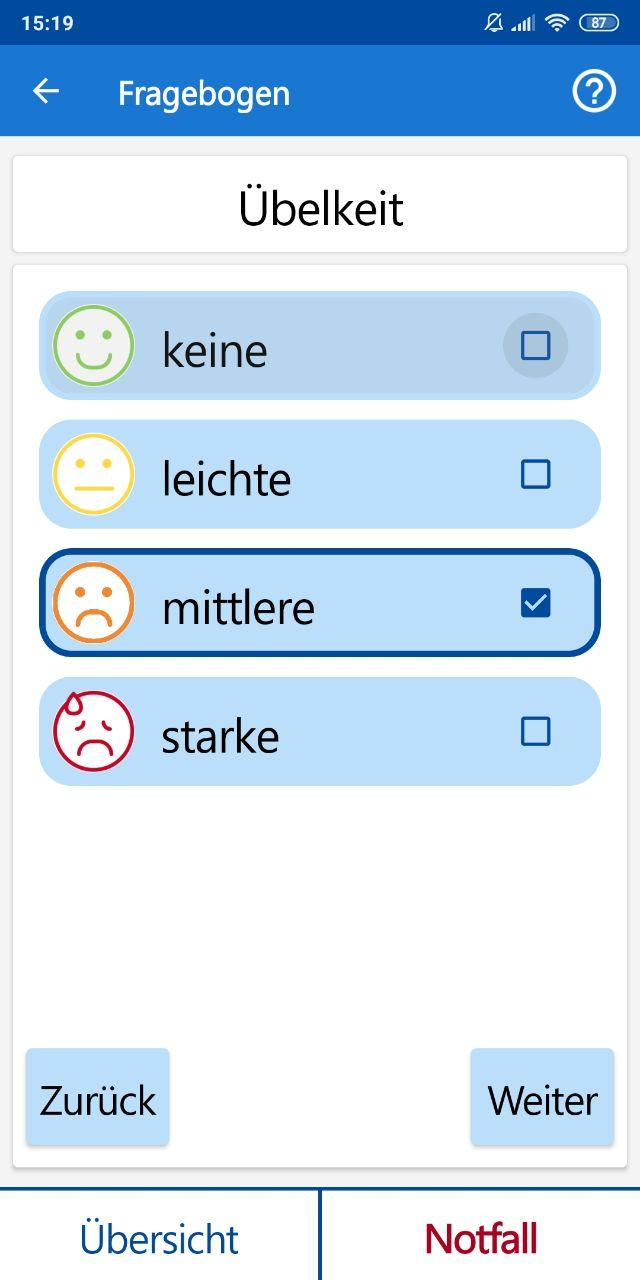
\includegraphics[width=0.28\textwidth]{figures/KlausMidos.jpg}
  \end{center}
  \caption{App version of the MIDOS survey}
  \label{fig:midos1}
  \vspace{-30pt}
\end{wrapfigure}
To achieve this, the user is guided through all questions like in a step by step tutorial. Examplary the first text is: "Bitte geben Sie an, wie stark heute Ihre Beschwerden sind." It is followed by multiple screens which look like the one in Figure \ref{fig:midos1}.
\subsection{Receiving data from a scale}
Apart from gathering psychometrical data with MIDOS, one essential functionality of our app is to acquire biometrical data of the patients through medical devices. In the first stage of our startup, we wanted to be able to demonstrate this functionality and decided to integrate a scale as proof-of-concept. One of our team members, Daniel, bought a scale from Beurer BF700\footnote{https://www.beurer.com/web/de/produkte/wellbeing/gewicht-und-diagnose/diagnosewaagen/bf-700.php} and connected to it with the help of the OpenScale project\footnote{https://github.com/oliexdev/openScale}. Since he  has taken up the task to create the webinterface, it was my job to complete the integration of the OpenScale code, and modify it to our needs. My idea was to modify the code as little as possible so 

\begin{wrapfigure}{r}{0.35\textwidth}
\vspace{-30pt}
  \begin{center}
  %TODO correct picture
    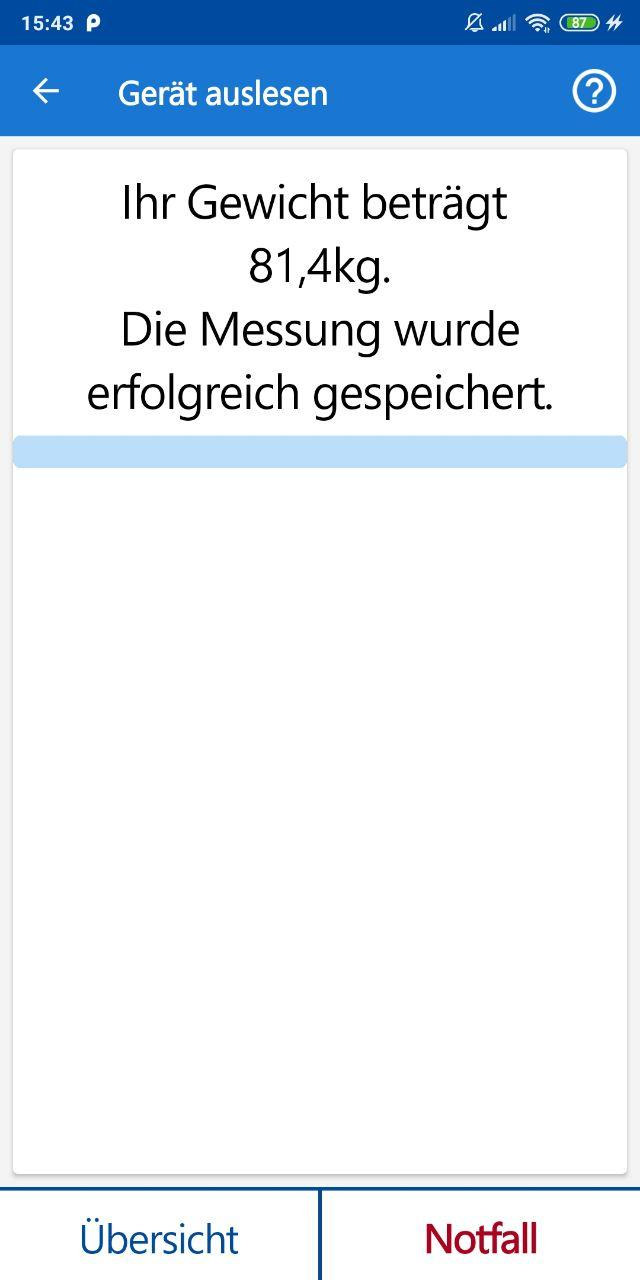
\includegraphics[width=0.28\textwidth]{figures/KlausScale.jpg}
  \end{center}
  \caption{Finished weighing}
  \label{fig:scale}
  \vspace{-10pt}
\end{wrapfigure}

that we would benefit from future updates of OpenScale without too much reworking. But yet some refactoring had to be done so that the app is reflecting the current state of the weighing process in a more adequate way. Therefore, we use a Handler as callback instance. It receives a Message object from the OpenScale classes and depending on the message state, a different action is executed. Since these messages are already sent before, during and at the end of the weighing process, we are able to lead a patient through the whole process. At first we advise the patient to switch on the scale and to step on it. After that a bar indicates the progress of the scaling and a visual, haptic (vibration) and auditive notification is raised when the weighing is done. After the process is finished, the weight is saved and displayed at the screen (see Figure \ref{fig:scale}). 
\section{Patrick Höfner}
\textbf{Responsibility: Back-End, Android-Development}\\
\textbf{Role: Wiki Master}\\

\subsection{Webserver}

To store the information collected via smartphone, a central storage location was required where the data could be stored persistently and made available to all communication partners. One central advantage of our system is to provide data-sovereignty on the patient side. This means that every health-care provider should be able to host a standalone system within his institution to guarantee that the collected patient-data can only accessed by a limited amount of trusted people.This trusted group has to be defined by the patient itself. The simplest and most cost-effective hardware to implement this project was a Raspberry Pi Model 3, which was provided by the university.
The Pi offered the necessary performance to process the data traffic and to host a web application. On the software side, the Raspberry Pi was installed with the operating system Raspbian\footnote{https://www.raspberrypi.org/downloads/raspbian/} in version 10 \glqq{}buster\grqq{}. This is a Linux distribution specially developed for the Pi and makes the best possible use of the limited hardware. A database management system was required to store, manage and process information. MariaDB\footnote{https://mariadb.org/} was chosen for this purpose. This provides a good compromise between performance and database features, such as security functions. In addition, the use of this software solution is classified as \glqq{}open-source\grqq{}, widely used and well documented, which was the most important selection criterion for rapid project progress.

To simplify database administration, PHPMyAdmin\footnote{https://www.phpmyadmin.net/} was installed, which provides a simple local web interface for database administration. Furthermore, an Apache web-server was installed, which will be used in the long run to access the website and database interface (API) via a browser. To realize such an interface a backend was needed which processes all database requests of the web and Android application and performs the necessary operations on the database. For this purpose the Django framework was chosen. This framework integrates important features like an authentication system with users and roles, security features as well as predefined libraries for the creation of database interfaces. The physical web server was installed on a Fritzbox 7530 in the apartment of a team member. 

However, there were some challenges to make the server accessible via the Internet. After several failed attempts, it turned out that most providers only assign IPv6 addresses, which led to accessibility problems. Thus the server was only accessible via devices which assigned an IPv6 address themselves. After a long search for a solution, this issue could be solved at least temporarily via a free service. The service named "ngrok"\footnote{https://ngrok.com/} provides a secure tunnel and a domain to make local web servers accessible via the Internet. Under the provided URL the server could be reached by all devices. However, this is not an appropriate solution in the long run, since the use of this external service should only be used for test purposes. This means the application should be accessible via the Apache web-server over a structured and well understandable domain. Moreover there should be installed dedicated security certificates for our web-service.


\subsection{Database Schema}
A database schema was designed to store the data in the database in a structured manner and to ensure that the integrity of the stored data is guaranteed. Due to the complexity of the application context, a number of database objects had to be considered. The basic concept of the database design is based on the assumption that all database objects can be uniquely assigned to one user. This database design originates from the authentication concept of the Django framework. There a so-called "user-model" is implemented, which can be assigned different roles and rights. Roles would be patients, doctors and relatives in the concrete use case. 


\begin{figure}[h]
    \centering
    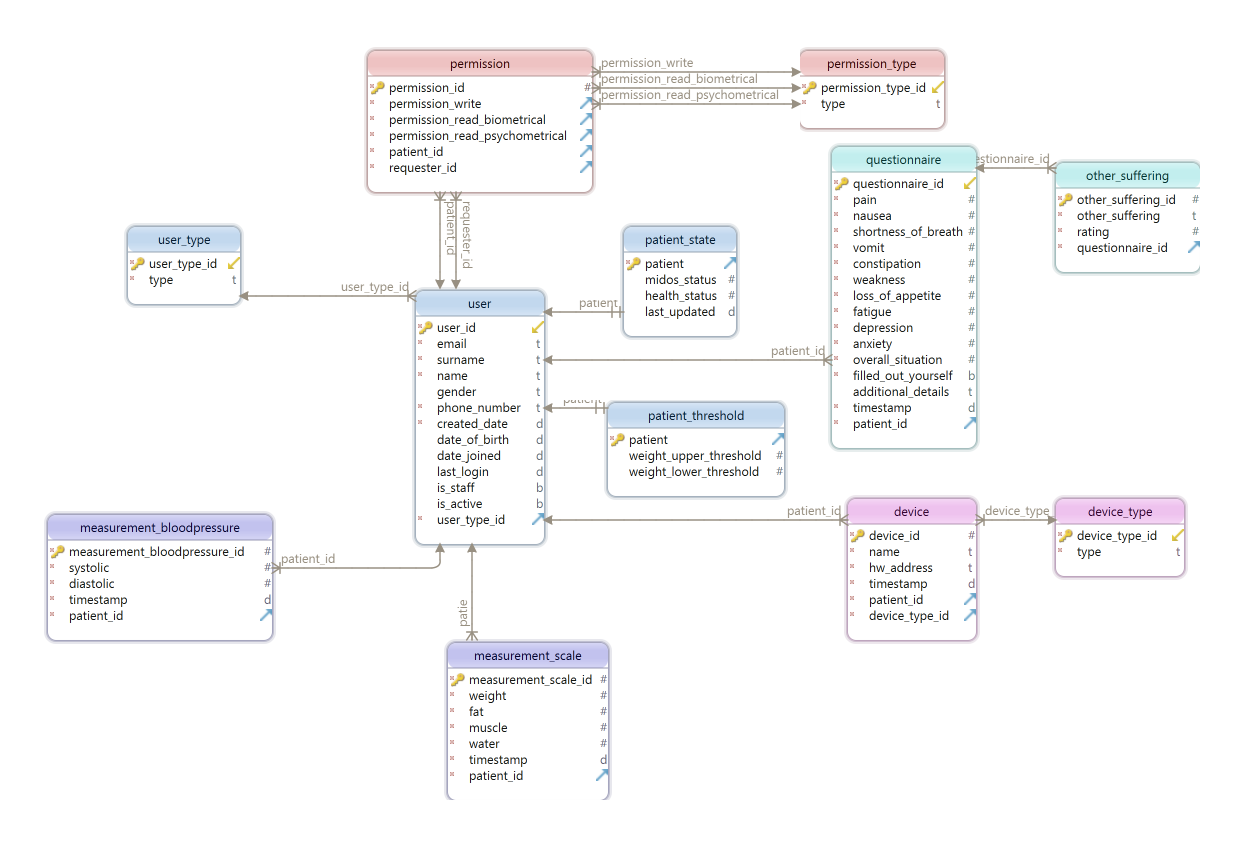
\includegraphics[width = \textwidth]{figures/dataScheme_Bericht.png}
    \caption[Database schema]{Database schema}
    \label{fig:DBSchema}
\end{figure}

However, a semantic problem arose when using this approach, since doctors and relatives do not create their own data records for measurements or completed questionnaires, but only access existing data records of specific patients. This problem was solved with an additional table "Permission", which determines which "user" is authorized to access the data of another "user". The "Permission" table also determines the depth of authorization. Additionally there are tables for "patient-state" and "patient-threshold". Therefore the state of a patient gets calculated and stored in the database depending on the thresholds which are set individually for each patient by the doctor. The database schema was created with the software "DBSchema"\footnote{https://dbschema.com/}, which made it possible to display the schema graphically, which was especially advantageous for the communication within the project team (see Figure \ref{fig:DBSchema}). In addition, the schema could be exported as ".sql" file and directly uploaded to the server as database via the PHPMyAdmin interface. Moreover the database was normalized into third normal form. This was important to avoid duplicates and to provide referential integrity. This means for instance, that only user types can be assigned to a user which have been predefined within the user-type table.


In the next step the database was connected to the Django backend. The Django framework is based on the Python programming language, which means that all operations to be performed on the database objects are also programmed in Python. This offers an enormous advantage from the developer's point of view, since no individual SQL statements have to be programmed. Conversely, however, this means that the tables of the MariaDB database must first be translated into Python objects so that the database entries can be accessed via Python code. Django uses a so-called \glqq{}Object-Relational-Mapper\grqq{} to translate existing SQL databases into Python objects, called "models"\footnote{https://docs.djangoproject.com/en/3.0/topics/db/models/}, which represent database tables. Once the database is migrated, the Django framework translates the Python commands into SQL and performs the desired operations on the database. 

\subsection{Visualization of biometric and psychometric information}
The visualization of the measured values for the user was realized by a series of activities, which all have the same basic structure. In defining a uniform structure, the focus was primarily on a simple, clear and comprehensible way of displaying the most important information to a patient without detours. When considering which information is most meaningful for the patient, after discussion and taking user feedback into account, the conclusion was reached that a temporal course of the measured values as well as an average value over a certain time is most informative for the patient. Therefore a basic layout was created for each activity, which implements a tab layout at the top of the screen. This enables the patient to display a time history over a week, a month or a year. The values are displayed using different types of graphs, which are adapted to the information displayed, and implement a red line for a maximum value that can be defined by a doctor in advance (see Figure \ref{fig:Screenshot1} a,b; \ref{fig:Screenshot2} b).

\begin{figure}[ht]
    \centering
    \subfigure[Weight activity]{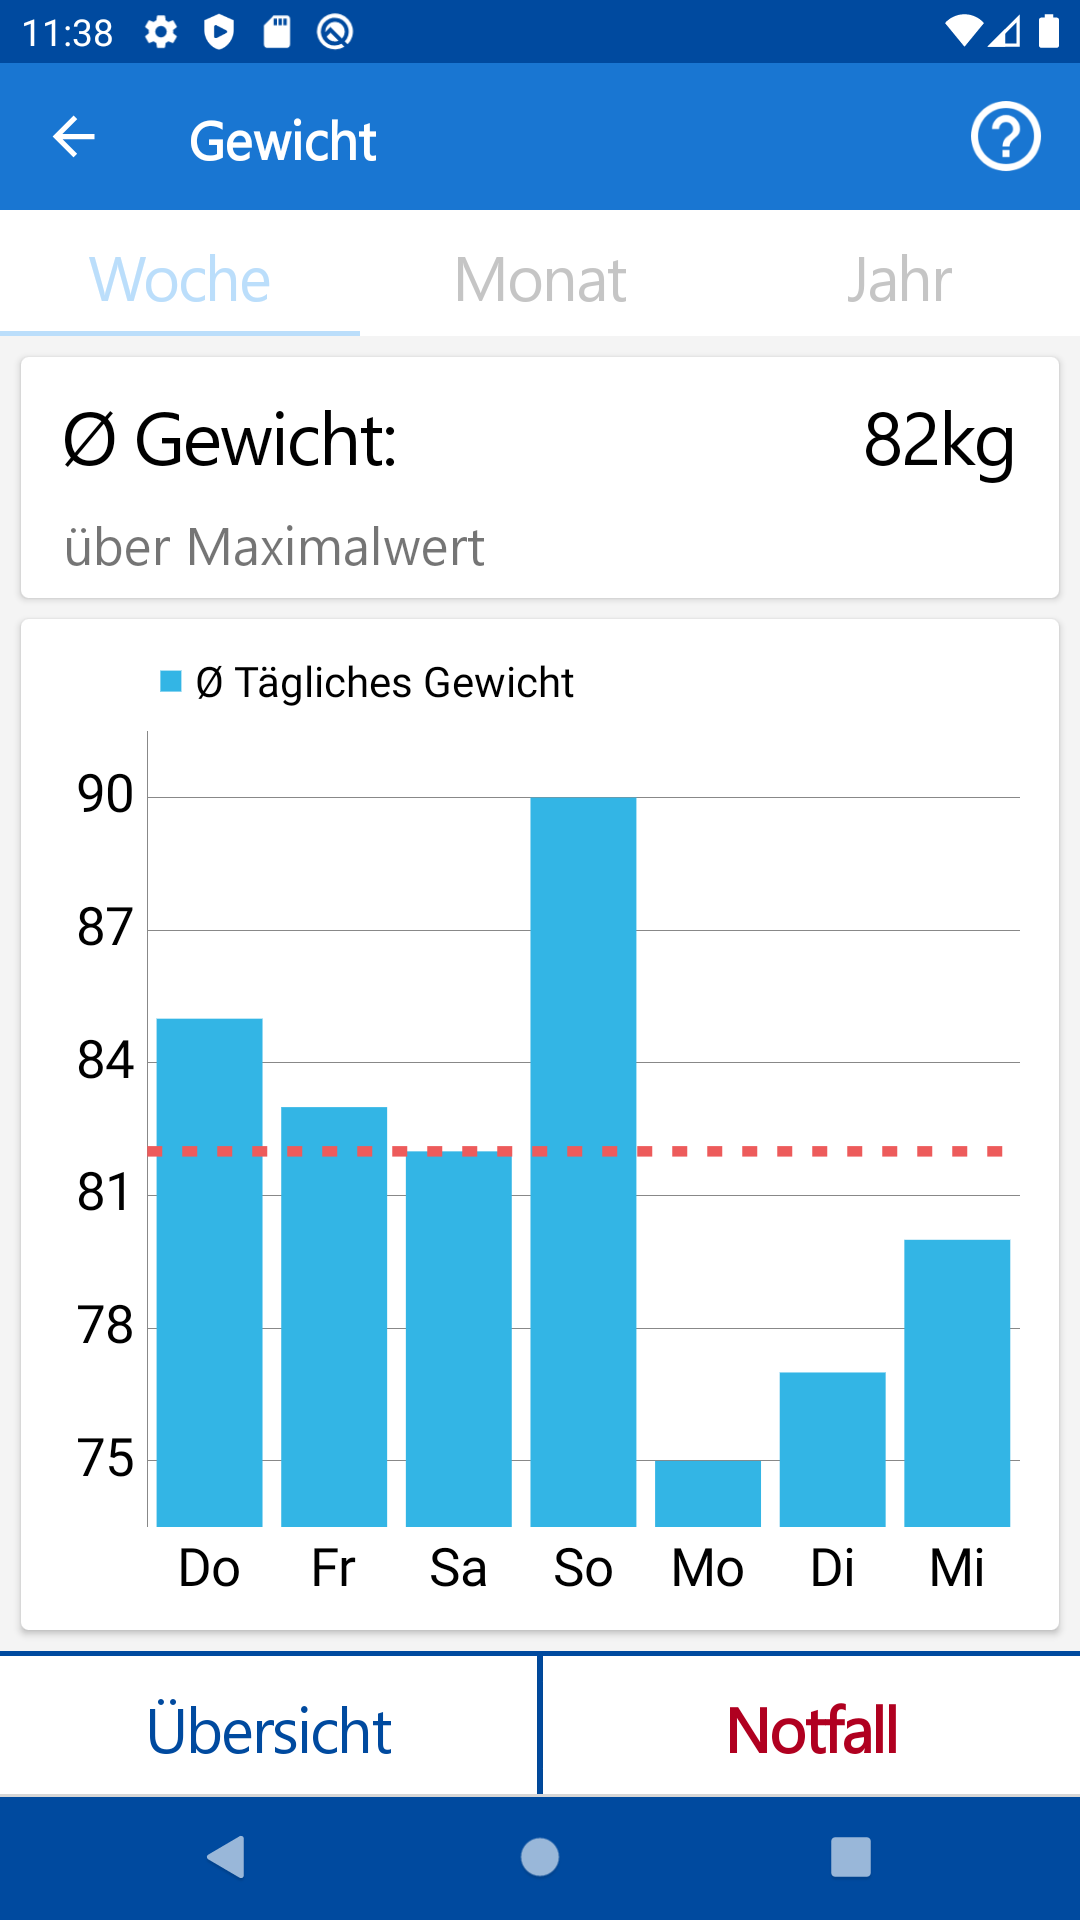
\includegraphics[width=0.30\textwidth]{figures/Screenshot_1584112496.png}}
    \subfigure[Bloodpressure activity]{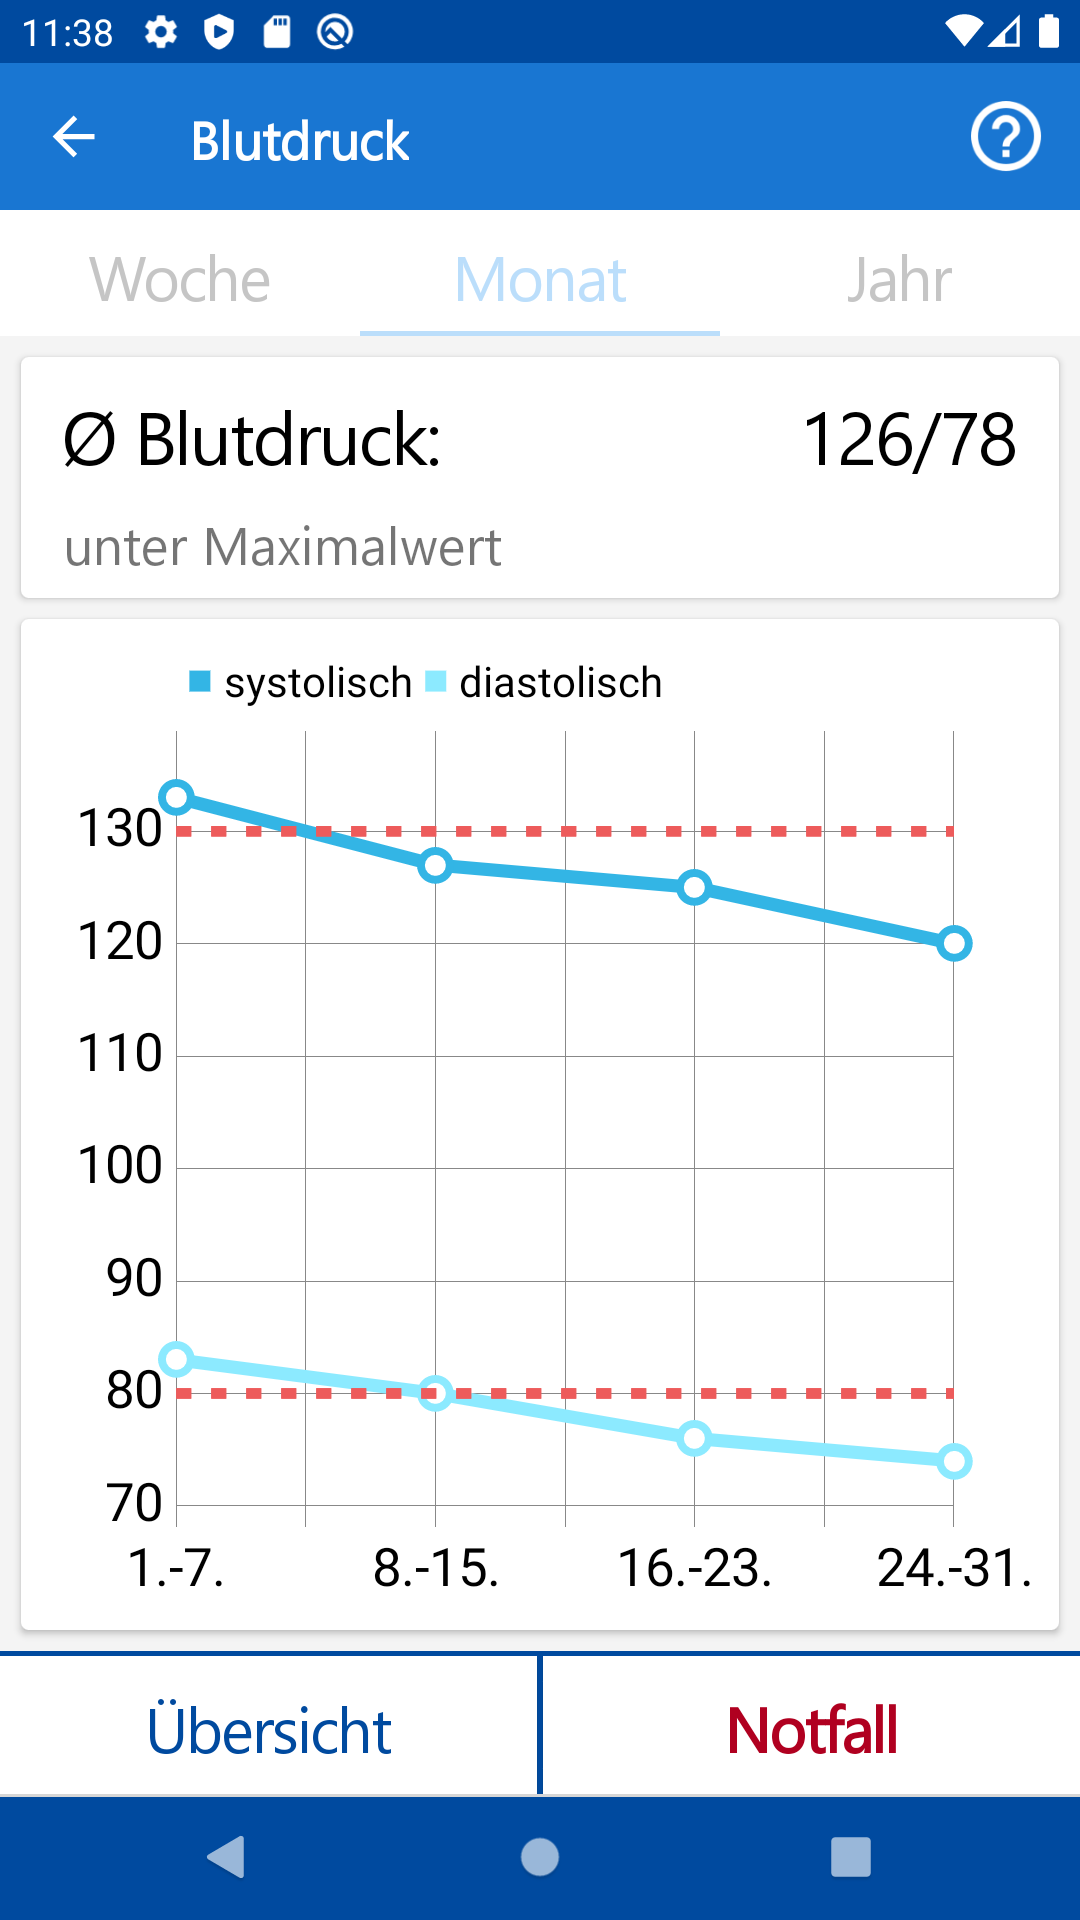
\includegraphics[width=0.30\textwidth]{figures/Screenshot_1584112512.png}}
    \caption[Screenshots of activities displaying biometrical information to the user]{\tabular[t]{@{}l@{}}Screenshots of activities displaying biometrical information to the user \endtabular}
    \label{fig:Screenshot1}
\end{figure}

The library \glqq{}MPAndroidChart\grqq{}\footnote{https://github.com/PhilJay/MPAndroidChart} was used to display graphs in the Android application. This library provides a number of very flexible customizable graphs and offers a good overall package due to its variety and good documentation. After the github repository was integrated into the Android project, all available functions of this library could be used. All values and value limits of the x- and y-axis are freely customizable which allows to display qualitative values. First of all, the display of biometric values - blood pressure and weight - was taken into account during the development, since the first development steps focused on the recording of data via the scales. For the display of weight we decided to use a bar chart because of the easy interpretation of quantitative values and the good recognizability of a time sequence (see Figure \ref{fig:Screenshot1} a). In order to display blood pressure, two related values are needed, the systolic and diastolic values. Therefore a line chart was used to display the blood pressure (see Figure \ref{fig:Screenshot1} b). Since the two values always have a distance between them, overlapping of the lines is impossible. Furthermore, the arrangement of the two related values on top of each other and auxiliary lines in the graph make it possible for the user to recognize relations.

\begin{figure}[h!]
    \centering
    \subfigure[Sufferings overview]{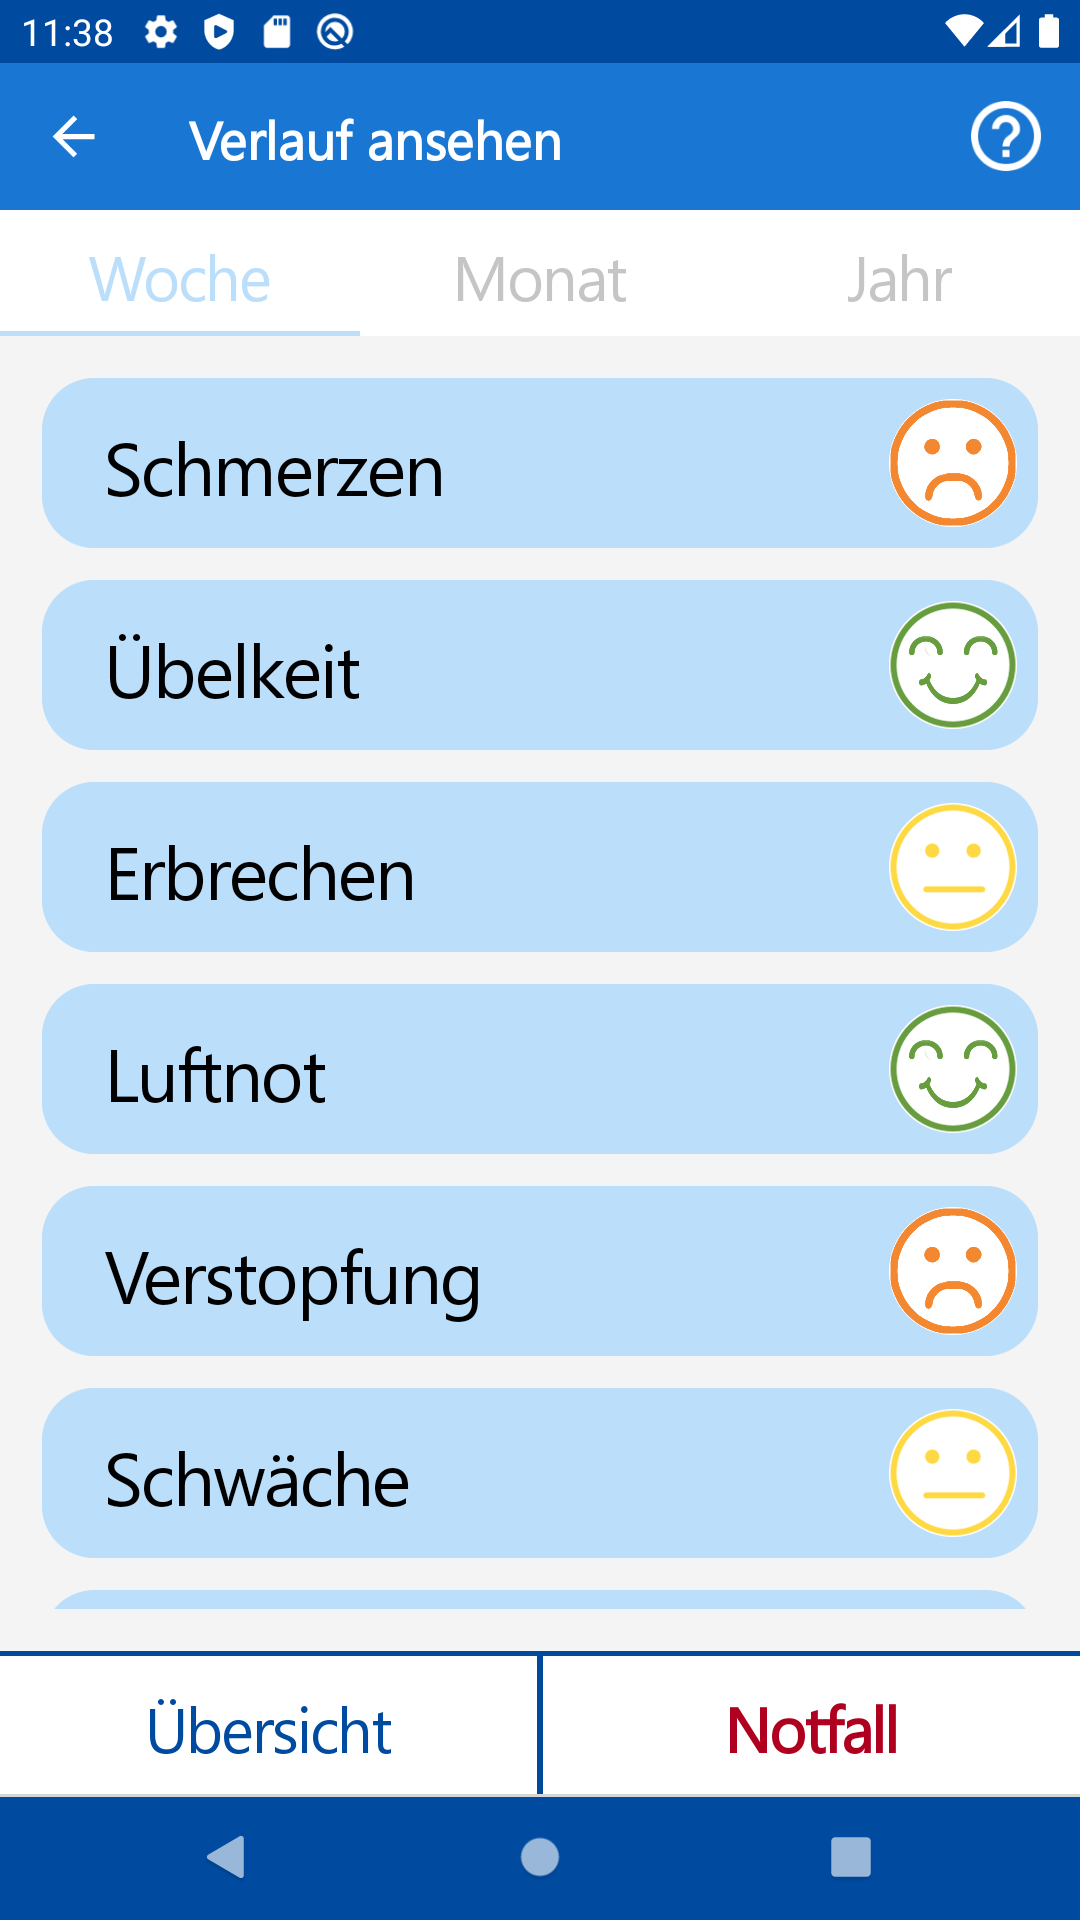
\includegraphics[width=0.30\textwidth]{figures/Screenshot_1584112527.png}}
    \subfigure[Sufferings detailed view]{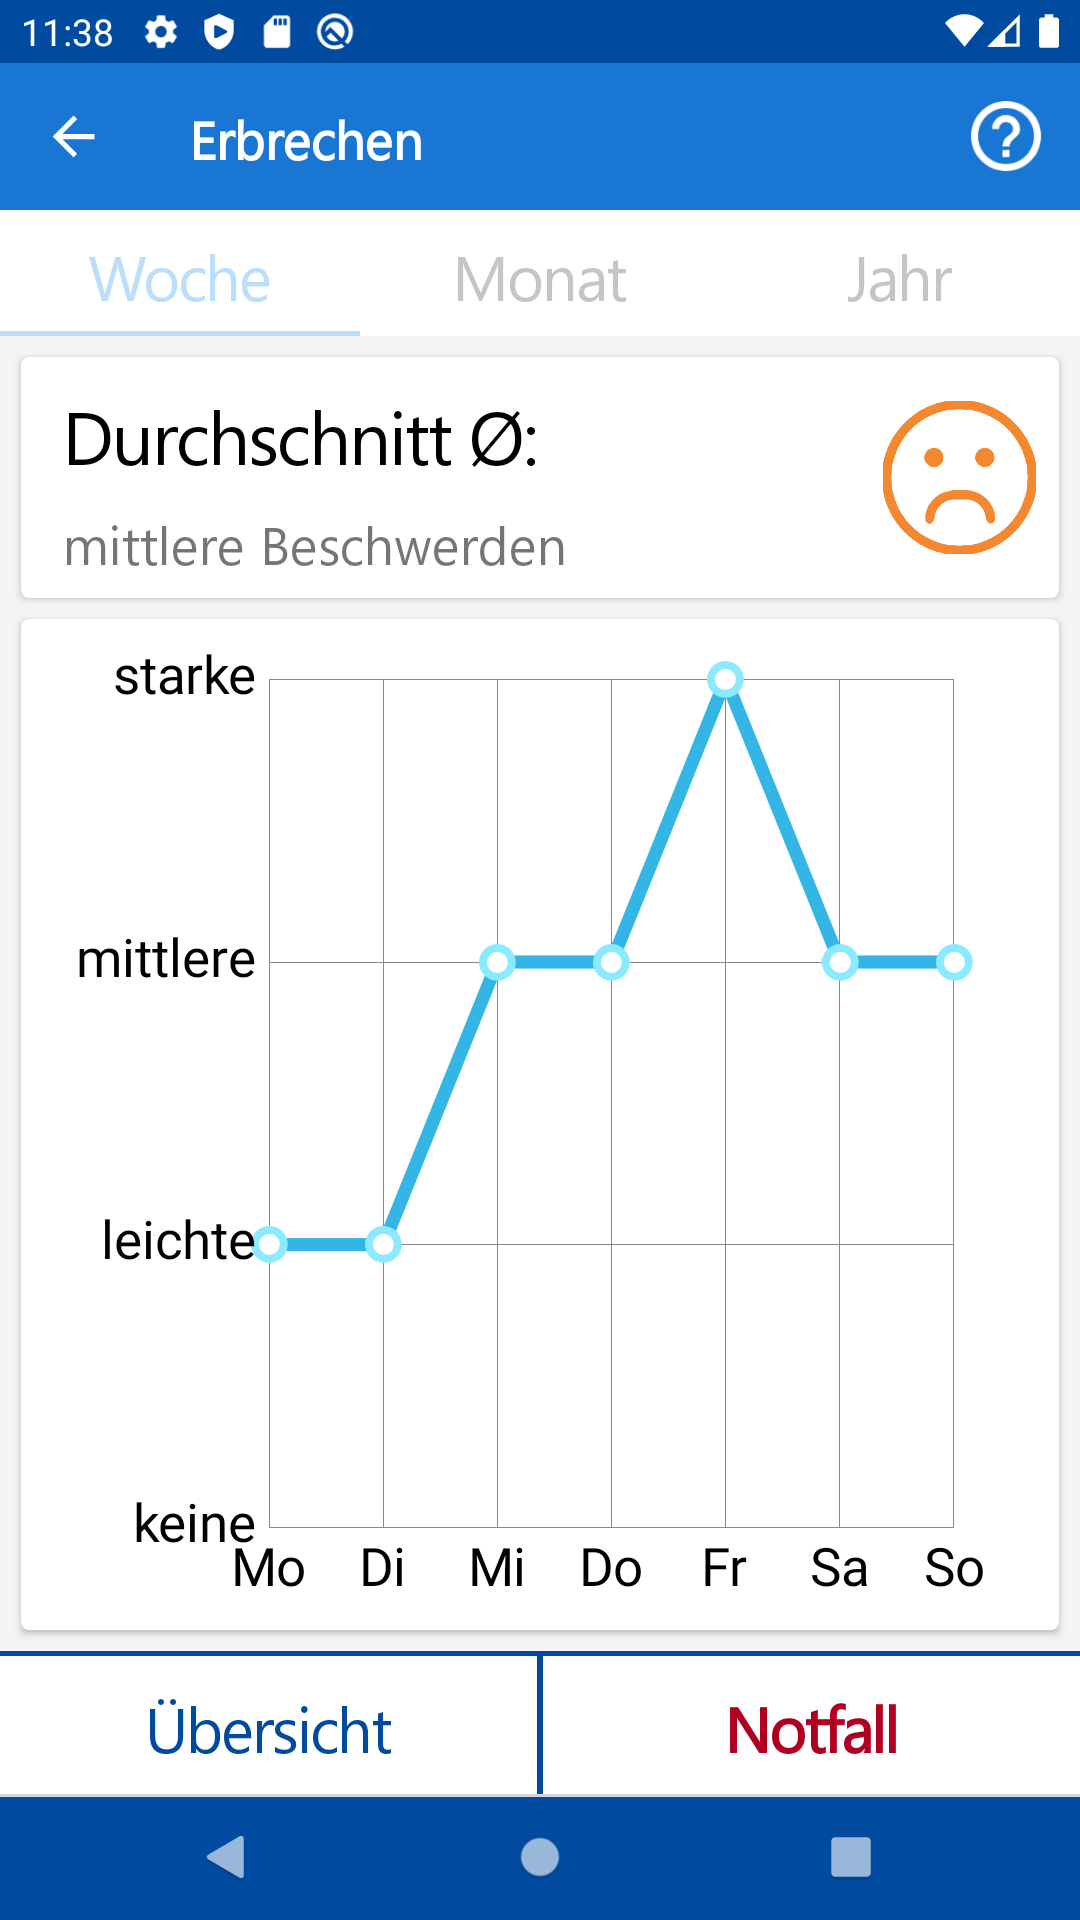
\includegraphics[width=0.30\textwidth]{figures/Screenshot_1584112570.png}}
    \caption[Screenshots of activities displaying psychometric information to the user]{\tabular[t]{@{}l@{}}Screenshots of activities displaying psychometric information to the user \endtabular}
    \label{fig:Screenshot2}
\end{figure}

Since problems with clarity arose when displaying all days of a calendar month or all months of a year due to the limited screen size, certain periods were combined. This means, for example, that in the year view an average value for the months January to March is shown in the graph and the individual months are not shown broken down for themselves (see Figure \ref{fig:Screenshot1} b). When implementing a view for the psychometric data, an additional overview activity was integrated, which provides an overview of all the conditions recorded in the questionnaire. Here the patient can see at first glance whether the recorded complaints were non-existent, mild, moderate or severe. Also in this view a certain period of time can be selected for the view via the Tab-layout (see Figure \ref{fig:Screenshot2} a). If a patient would like to get more detailed information about a certain ailment, he can click on the respective button to get to the detailed view. There, analogous to the biometric information, a line chart is displayed, whereby a line chart was chosen based on the qualitative values (see Figure \ref{fig:Screenshot2} b). 

\subsection{REST-API}
Django REST framework\footnote{https://www.django-rest-framework.org/} was used to store and retrieve data on the server via the internet. It can be seamlessly integrated into Django and provides the most important functions for defining an Application Programming Interface (API). API defines a set of endpoints that can be used to perform certain operations on the server's database by using backend functionality. Each endpoint is assigned its own domain, through which certain information can be retrieved or stored. Within the project, so-called GET and POST requests were used, which are sent from the client to the server.  This could be managed by implementing the libary "Retrofit"\footnote{https://square.github.io/retrofit/} within the Android application which will be explained in further detail later on. With a GET-request data can be retrieved from the server and with a POST-request a new data set can be created on the server. The JSON\footnote{https://www.json.org/json-en.html} data format is used to transfer data records structured in text form and to interpret them correctly afterwards (see Figure \ref{fig:ClientServer}). 

To ensure successful communication between Android application, server and web application, endpoints for the registration of a new user and the login/logout of an existing user were defined. The Django framework provides predefined functionality to generate a token after successful registration or login, which is needed to retrieve or store data from the server.
The token authentication ensures that only authorized, i.e. registered and logged in users, have access to the data. Due to the individual adaptations of the standard Django user model, a number of adjustments were also necessary when using the given functionality of the Django-REST-Famework. Besides registration and login endpoints, there were defined endpoints to access data about users, patient-status and questionnaires.

\begin{figure}[h]
    \centering
    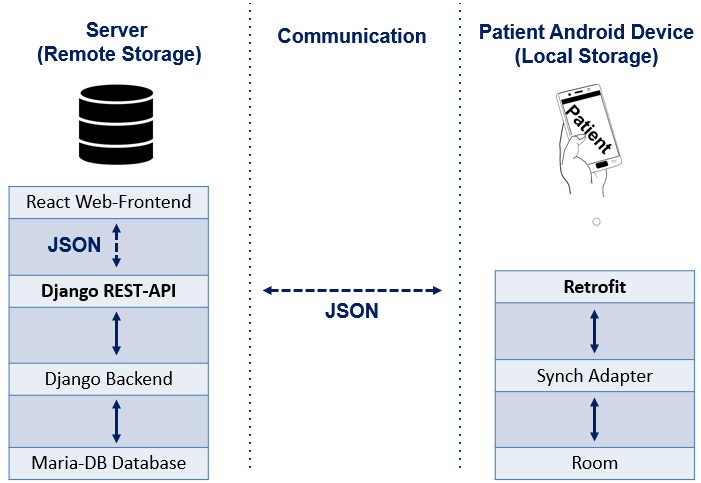
\includegraphics[width = \textwidth]{figures/Client-Server-Architecture.png}
    \caption[Database schema]{Description of the client-server-architecture}
    \label{fig:ClientServer}
\end{figure}
\section{Ulla Sternemann}
\textbf{Responsibility: Android App Database}\\
\textbf{Role: Scrumboard Master}\\

\subsection{Databases in Android applications}

As we need to store the user's personal data as well as all acquired biometric and psychometric information, the Android application needs to handle large amounts of structured data. Therefore, it is necessary to implement a private database for our app. 
Additionally, not only the patient has to be able to access his or her collected data, but it also has to be shared with all other communication partners, which are for example members of SAPC teams, general practitioners, or next of kin. Eventually, the goal here is to provide every user at every time with the requested data. 

Accordingly, the smartphone app needs a suitable database architecture that provides the option of local and persistent data storage and synchronization with the global database on the webserver. 

There are different options to implement a database within an Android application. The most common ones are using either an \textit{SQLite}\footnote{https://www.sqlite.org/index.html} database or the \textit{Room Persistence Library}\footnote{https://developer.android.com/topic/libraries/architecture/room}. 

The Room Persistence Library is part of the \textit{Android Jetpack}\footnote{https://developer.android.com/jetpack}, which is a collection of Android software components that can be used for fundamental functionalities of the app, such as lifecycle management or database development. 

Room provides an abstraction layer over SQLite and allows fluent database access. Using only SQLite, we would need a lot of boilerplate code to convert SQL (Structured Query Language) queries to Java data objects \cite{wei2012android}. Room takes care of that problem because it maps database objects to Java objects without boilerplate code. Moreover, Room provides verification of raw SQL queries at compile-time which preserves the app from crashes at run-time due to incorrect SQL queries. Also, to be able to enter and view their data at every time, it is important that the users of our app can access the database even if its not possible to establish a connection to the server. Therefore, the app has to persist relevant parts of the data in a local cache. If there are any data changes during the offline time this new data then has to be synchronized with the database on the server \cite{room1}. As the Room library takes over all these tasks, we chose to use it for the database of our Android app. 

\subsection{Database implementation using \textit{Room}}

\subsubsection{Architecture of a Room database}

Every Room database consists of several different components. The three major ones are Entities, DAOs (Data Access Objects), and the Room Database itself. The corresponding classes are tagged with special annotations (\texttt{@Entity}, \texttt{@Dao}, \texttt{@Database}) to mark them as database classes. The following part describes the different components and how each of them is used which is also described in Figure \ref{fig:room_architecture}. 
\begin{itemize}
	\item \textbf{Entity} \\
	Each class annotated with \texttt{@Entity} represents a table within the database. The fields of these classes are the columns of the corresponding tables. Also, foreign keys, primary keys, and relations can be defined within the entity class. 
	
	\item \textbf{DAO} \\
	Each class annotated with \texttt{@Dao} represents an interface which defines the mapping between SQL code and Java functions for database access, such as inserting, updating, deleting, or querying data. Each DAO is associated with one entity. 

	\item \textbf{Database} \\
	The class annotated with \texttt{@Database} represents the main access point for the connection to the underlying SQLite database. Within this class, all entities and DAOs which belong to the app's database are listed. 
\end{itemize}

The app uses the database class as the only entry point to the database. Through the database class, the app gets access to all DAOs, which are the connection to the entities associated with that database. Using the functions of the corresponding DAO, the app can access and modify the data, which means getting and setting field values of the entity \cite{room1, room2}.

\begin{figure}[htb]
	\centering
	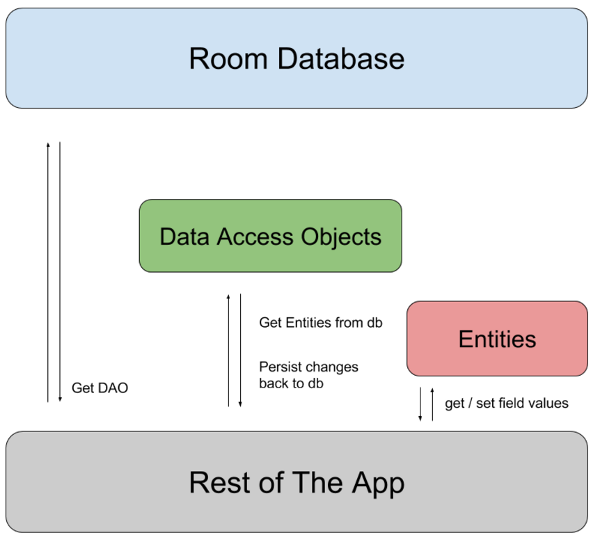
\includegraphics[width = 0.7\textwidth]{figures/room_architecture.png}
	\caption[Room architecture]{Architecture of Android Room database\footnote{https://medium.com/mindorks/using-room-database-android-jetpack-675a89a0e942}}
	\label{fig:room_architecture}
\end{figure}

% 3 richtige quelle https://developer.android.com/training/data-storage/room


\subsubsection{Communication of database and UI}

As the user of our app should always be able to view an up-to-date version of his or her data, we need to make sure that the apps UI (User Interface) state matches the state of the data which is contained in the database. Accordingly, when performing queries, for example when the user is looking at the app screen which shows the blood pressure or weight graphs, the UI should display the currently correct data and update automatically when this data changes. Therefore, so-called observes are used. Anytime the state of an observed object changes, for example if a table in the database is updated, all observers which are bound to that object are notified and hence can take care of adapting the UI. 

For this purpose, we use \textit{LiveData}\footnote{https://developer.android.com/topic/libraries/architecture/livedata} and \textit{ViewModel}\footnote{https://developer.android.com/topic/libraries/architecture/viewmodel} objects, and an additional repository class as this is common best practice to handle the data communication between a Room database and the app's UI. The following explains the different components and how each of them is used. That is also described in Figure \ref{fig:room_livedata}. 

\begin{itemize}
	\item \textbf{LiveData} \\
	When there are changes in the data, the Room library takes care of updating all LiveData objects, which are observable data holders. Also, LiveData objects are lifecycle-aware, which means that they are aware of the current lifecycle status and relevant lifecycle status changes of the corresponding UI class. Consequently, UI components such as Activities or Fragments observe only relevant data and update only if they are currently in an active lifecycle state. 
	
	\item \textbf{ViewModel} \\
	A ViewModel object acts as the communicating element between the database repository and the UI. The ViewModel holds all the data which is relevant for one UI component wrapped in LiveData objects which take care of updating the data if it is necessary, as explained above. Hence, the UI components no longer have to take care of getting the data as the correct data is always stored in the ViewModel. Additionally, ViewModel objects survive configuration changes of UI components like for example device rotation and are therefore able to always provide the UI with the necessary data. 
	
	\item \textbf{Repository} \\
	The repository class provides a clean API for data access and is the single source of truth for all app data. It is used to manage multiple backend data sources, considering our app these are the global database on the server and the local Room database on the phone. The repository defines the logic for deciding whether to use locally stored data or to fetch data from the server. Also, it handles appropriate threading of database access as such operations have to run on separate threads to avoid blocking the main UI thread with for example long-running database queries. 

\end{itemize}

\begin{figure}[htb]
	\centering
	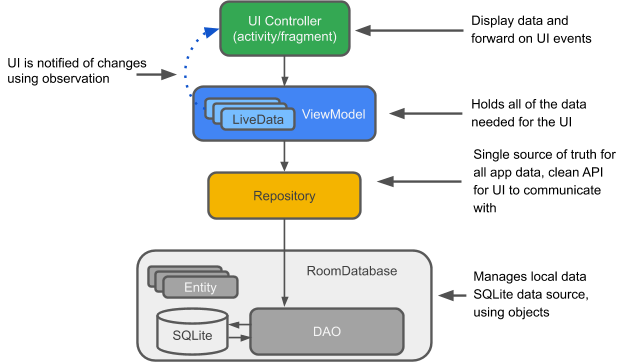
\includegraphics[width = \textwidth]{figures/room_livedata.png}
	\caption[Communication of database and UI]{Communication of database and UI\footnote{https://codelabs.developers.google.com/codelabs/android-room-with-a-view-kotlin}}
	\label{fig:room_livedata}
\end{figure}

In summary, the app uses LiveData objects which take care of observing data changes and updating the currently active UI components with the relevant data if it is necessary. The corresponding data for the UI components is held by ViewModels which are responsible for always providing the up-to-date data to the UI, even during configuration changes. 

There are several advantages of using this combination of architecture components for database-UI-communication. First, manual lifecycle handling it unnecessary and hence, less boilerplate code is needed. In addition, app crashes due to stopped or destroyed Activities and Fragments are avoided as only active UI components are updated. As a result, the UI matches the data status at any time, because all UI components automatically receive the latest data immediately after they come to the foreground and thus are visible for the user \cite{livedata1, livedata2}. 

\subsection{Data synchronization using \textit{Retrofit}}

A major advantage of our system is that the patients' data can be shared with the other types of users, namely next of kin, doctors, and SAPC team members, to ensure that they are always informed about the patient's health status. For example, the SAPC teams can use our web application to monitor the condition of all patients assigned to them. Therefore, synchronization of data between Android devices and our global database on our web server is necessary to make all the needed information available to all different kinds of users of our system. For this purpose, we use the \textit{Retrofit HTTP client}\footnote{https://square.github.io/retrofit/}.

Retrofit is a type-safe HTTP client for Android. The library provides a powerful framework for authenticating and interacting with APIs and sending network requests. Moreover, retrieving and uploading JSON files via a REST-based web service is fairly straightforward. Retrofit maps an HTTP API to a Java interface within our Android app. This is made possible by parsing JSON files, on which the communication with the database located on the webserver is based, into POJOs (Plain Old Java Objects). The resulting POJOs can then be fed into the local Room database \cite{retrofit1, retrofit2}.

To be able to issue network requests to a REST API with Retrofit, API endpoints need to be defined inside of a Java interface. Therefore, Retrofit annotations are used to encode details about the HTTP request method, the parameters, and the method used to dispatch the network call. Also, the relative URL needs to be defined. Examples for such Retrofit annotations are \texttt{@GET} or \texttt{@POST}. This works similar to the mapping of SQL queries to Java function within the DAO interfaces for Room database \cite{retrofit1}. 

Using the Retrofit HTTP client has several advantages compared to developing an own server app communication. It is ideal for use-cases where direct communication with the webserver is intended which is the case for our system. As Retrofit takes care of converting JSON files to POJOs there is no need for manually defining the parsing operation which makes using Retrofit very low effort. Furthermore, Retrofit allows asynchronous handling of server access operations which leads to better app performance as the server access does not block any other operations \cite{retrofit2}.


\section{Daniel Wagner}
\textbf{Responsibility: Scale sourcing, experimental scale integration, web-app frontend and  backend}\\
\textbf{Role: Communication Master}\\

\subsection{Scale sourcing}

To develop a proof of concept it was required to show 3rd party medical devices could be integrated into our system. For this purpose, we decided to use either blood pressure measurement devices or body analysis scales. The reason for choosing those device categories is that relatively speaking they are simpler to integrate into a project that is supposed to be built upon none proprietary hardware, firmware and software while at the same time still having the capability to capture relevant medical data for our use case [1.2]. We further narrowed down our scope of relevant devices by conversing with our project owner and medical professional Tobias Steigleder. We then screened Opensource code platforms and forums for code that would allow us to integrate some of these devices. Based on the ability to be integrated into our project and other criteria like price, market availability and quality of measurements the following devices made it into our closer selection:

Respiratory Rate / Blood pressure:

\begin{itemize}
	\item Soehnle Blood Pressure Monitor Systo Monitor Connect 300

	\item Omron RS7 Intelli IT Wrist Blood Pressure Monitor

	\item Beurer BM 54 Bluetooth Blood Pressure Monitor
\end{itemize}

Weight/ Body composition:

\begin{itemize}
	\item Kamtron Bluetooth Digital Personal Scales

	\item Vigorun Smart Bluetooth Electronic Body Fat Scales

	\item Beurer BF 700 Diagnostic Bathroom Scales\\

\end{itemize}

Subsequently tests in a local technology store could be performed to further assess the viability of the devices pre-purchase. However not just the devices above were tested but the whole sortiment of the Mediamarkt and Expert stores. The tests were performed by using the Nordic Semiconductor nRF Connect app as well as the development version of the Openscale app\footnote{https://github.com/oliexdev/openScale}. The tests were performed with phones that used different physical layers (phy1M and phy2M) as this can have an impact on the signals that are being received on the host device. This knowledge is based on previous experience with the ESP32 microcontroller and experiments with different android phones. Other factors to consider are turning on location services on the phones when trying to connect to a Bluetooth Low Energy (=BLE) device. It is recommended to install the manufacturers app to establish the first connection to the BLE server device (scale). After connecting for the first time the manufacturer apps should be closed as they can interfere with the debugging apps and the phone system as they usually are very unstable or do not work at all on some devices. Debugging the BLE connection which involved reading out characteristics and services with the nRF Connect app became possible for most scales that supported BLE. Testing scales with the openscale project was only feasible for scales that were supported. 

In the end the Beurer BF700 was chosen for the following reasons:

\begin{itemize}
	\item internal measurement cache with support for different profiles and the ability to delete all data

	\item existing documentation and support in Open Scale project as well as positive comments on the project page for this particular scale

	\item 5 years warranty and good brand reputability

	\item intuitive measurement procedure for weight, fat, hydration all in one and different Bluetooth Low Energy data streams for the respective measurement

	\item one of the best manufacturer apps
\end{itemize}

\subsection{Experimental scale integration}

Gray box testing was performed on the Openscale code to understand its functionality, find potential bugs and identify the pieces that could be used for our own project. First the whole app was segmented, analyzed and sequentially stripped from the modules that were not essential to realizing a BLE connection and receiving data. This turned out to be difficult as the author very tightly coupled data management and BLE connection handling. The following mindmap shows the structure of the Openscale project, what components were used for the production build (orange) and for the development build (purple). All other components were ditched with the aim to create a lean app that with as few conflicts as possible with code that we wrote and Openscale code.

\begin{figure}[h]
	\centering
	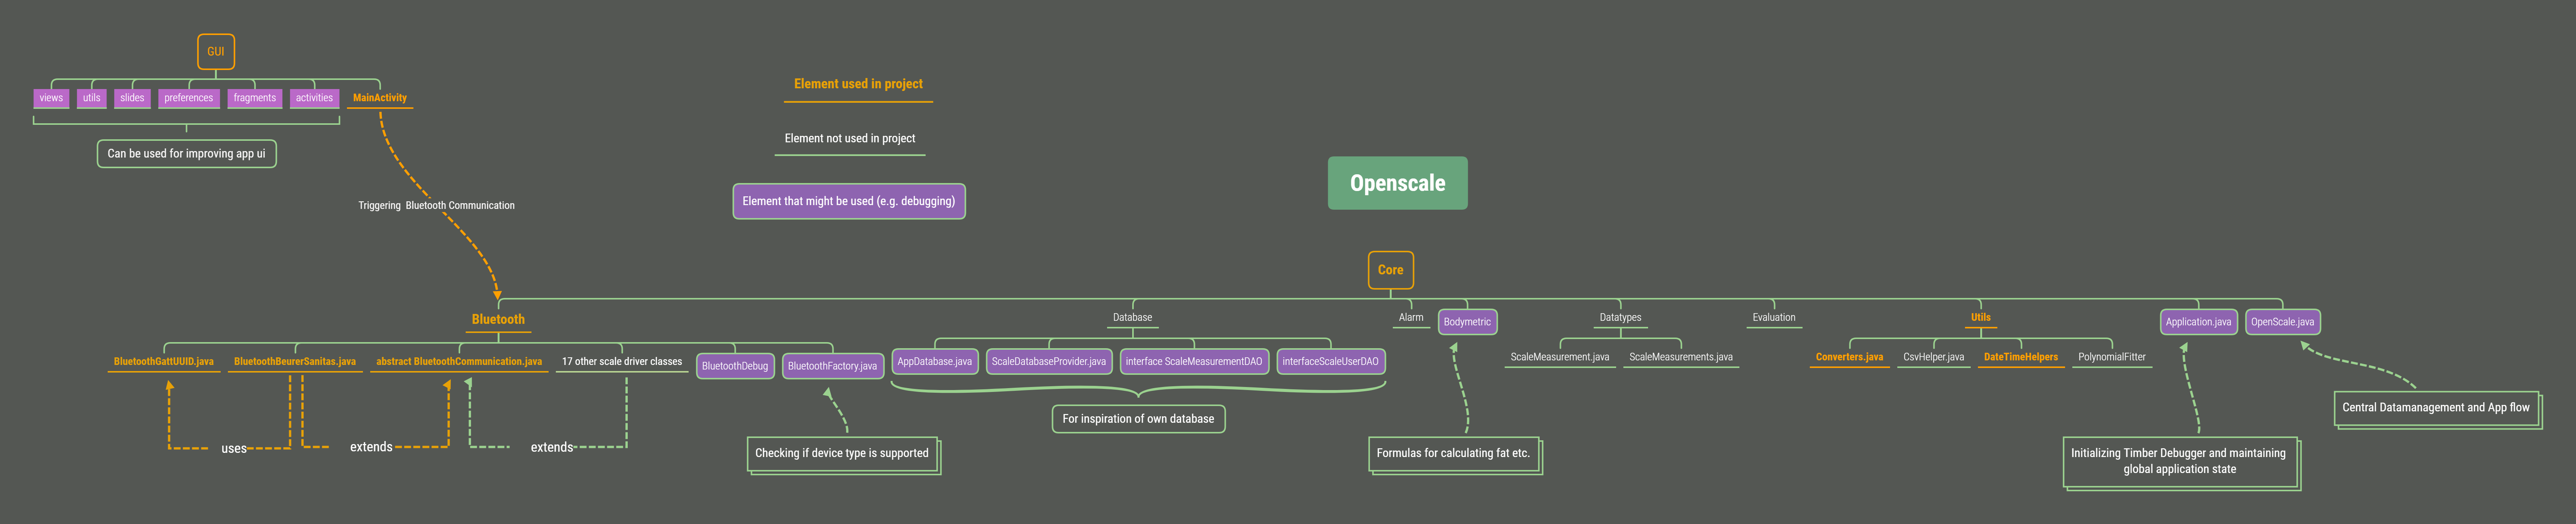
\includegraphics[width=\textwidth,height=2.0in]{./media/image1.png}
	\caption{Openscale project overview}
\end{figure}

\subsection{Setup of web-app project}

Our web project consisted of two parts. The backend should aggregate data from the patient ‘s phone app as well as relay this data back to any frontend that would display it. A few system design decisions were made for realizing this. The backend framework we used was Django which suited itsself to our team as some members had previous experience with it and it quickly allows you to get started. Other reasons for choosing Django include that there is an active developer community, the fact that it is a well-maintained project and that there is a plethora of documentation available.

For the frontend React JS was chosen for mostly the same reasons as Django. Both work nicely together and there exist many projects that use the two technologies in tandem. The fundamental idea of the software stack is that Django would serve static files on a webserver. This included images, html, css and most importantly the compiled React Javascript code. Although not splitting frontend and backend into two seperate code bases might not be very common in software development, this allowed us to package the web-app more tightly. This also made a faster development workflow and fully leveraging Django ‘s capabilities possible.

Django ‘s functionality can be explained with the Model View Controller concept\footnote{https://djangobook.com/mdj2-django-structure/}. Essentially when a URL is called in the browser a method of a view object is triggered. The view can then make database calls via model objects and start executing code on the server. In our project we used views to perform authentication, load frontend code as well as loading and saving data to and from the backend.

\begin{figure}[h]
	\advance
	\leftskip 0.05in	
	\centering
	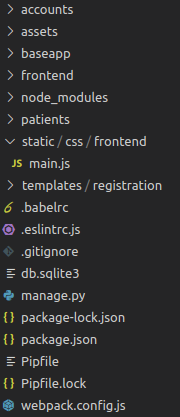
\includegraphics[width=1.87in,height=4.34in]{./media/image2.png} \caption{Web project folder structure}

\end{figure}

In Django different apps can be created to seperate functionality within the entire web app. Each app can define its own URLs that trigger the respective view method as well as the models that manage database functionality. The accounts app was used to expose an API for authentication. Assets stored image or animation files. Baseapp is the entry point for the entire project and is used to configure libraries, the behaviour and priority in which other Django apps are loaded as well as telling Django where certain files are located. Frontend is a placeholder app whose purpose it is to load the compiled React code. Patients manages all patient data and offers it in form of a REST API. Manage.py is the shell console with which all the Django server can be controlled. All other folders and files are used for frontend purposes. Node\_modules stores all React library modules. Static / css / frontend stores all compiled Javascript code that Django can serve via its frontend app. In templates html files (e.g. login forms) can be stored. .babelrc is the configuration file for Babel which is a compiler and syntax transformer for Javascript. It's main usage is to use newer syntax without waiting for browser support as the the compiled javascript becomes backwards compatible. package.json defines all libraries that should be loaded with Javascript package managers like npm. Pipfile defines all the python packages that should be loaded for Django. For this to work pipenv should be installed on the system. Lastly webpack.config.js is the config file for Webpack which compiles and bundles all frontend source code into one single file that Django can load and render websites with. 

\subsection{Backend development}

When a URL is called that points to the IP of the webserver the first thing that happens is that Django starts searching for a route in the ‘baseapp’ app urls.py file. First it checks whether the admin panel was called (127.0.0.1:8000/admin/). If this is not the case API calls for the patient REST API (127.0.0.1:8000/patients) or accounts authentication API (127.0.0.1:8000/auth) are handled first. Only after those are handled, Django will try to render the frontend (127.0.0.1:8000). This distinction is important so that Django does not try to handle API calls when no route is entered. \\

\textbf{Patients API}

This API was realized via the Django Rest Framework whose general functionality was described before (4.4). More specifically the ‘patients’ app defines all database fields that are managed in the models.py file. These fields are then converted to JSON with the serializers.py file. The api.py file then takes that JSON data and exposes all of it to the API endpoint (127.0.0.1:8000/patients).

When calling the API URL all patient data like midos status or health status can be accessed in one JSON object. \\

\begin{lstlisting}[label={lst:mylabel}, caption={'Patients' JSON object},captionpos=b, basicstyle=\small, tabsize=3]
	[
		{
			"id": 2,
			"first_name": "Adriana",
			"last_name": "C. Ocampo Uria",
			"last_update": "2019-12-21T15:18:26.666167Z",
			"midos_status": "good",
			"health_status": "medium"
		}, 
		{
			"id": 3,
			"first_name": "Edmond",
			"last_name": "Halley",
			"last_update": "2019-12-21T15:18:45.070093Z",
			"midos_status": "bad",
			"health_status": "medium"
		},
		{
			"id": 4,
			"first_name": "Gertrude",
			"last_name": "B. Elion",
			"last_update": "2019-12-21T15:18:55.977195Z",
			"midos_status": "critical",
			"health_status": "critical"
		},
		...
	]
\end{lstlisting}


\textbf{Authentication}

JSON Web Tokens\footnote{https://jwt.io/} (=JWT) were used for authentication and protection of the API endpoints. The ‘patients’ API can only be accessed when a token authentication has been performed. This is handled with three URLs: 127.0.0.1/auth/, 127.0.0.1/refresh/, 127.0.0.1/verify/. A token can be fetched by providing login credentials to the auth URL. Its expiration time is set to 5 minutes. The token needs to be refreshed in that interval. If this does not happen the API points cannot be accessed anymore. After refreshing, a new token is generated which can then be used to refresh again. Currently this authentication system is only used for the web-app. The biggest benefit of using JWT is however, that single-sign-on systems can be realized with it. Once a user is logged out or signed in this will be the case on all devices. This can be coupled with activity tracking (e.g. tracking whether a user clicks on buttons or moves mouse) on the device being used in the moment to create a very secure system and to keep the medical data of the patients protected. Having an activity tracking system that performs auto logouts alone does not secure the API endpoints. Therefore, a server-side authentication system is required. 

\subsection{Frontend development}

\textbf{Components}

\begin{figure}[h]
 	\centering
 	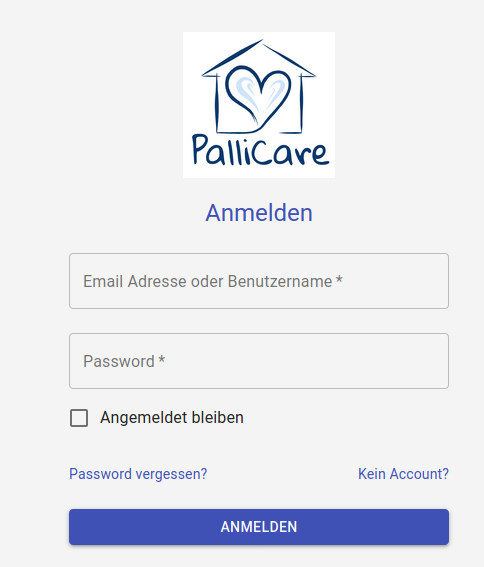
\includegraphics[width=2.65in,height=3.1in]{./media/image4.png}
 	\caption{Login screen}
\end{figure}


\begin{figure}[h]
	\centering
	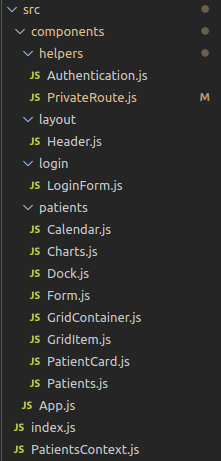
\includegraphics[width=1.7in,height=3.19in]{./media/image3.png}
	\caption{Component overview}
\end{figure}

One of React‘s most important features is its components system. Almost every function or part of the user interface will be handled by a react component. Components can have parents and children. This results in a component tree with components stacked in each other. The login screen of the app contains components that pass along information to a global context (username, password etc.). Within these components other components are nested like the image component for the logo, form components for the username and password as well as control components for the button.

On the mainscreen of the app cards were built using the material design library\footnote{https://material-ui.com/}. With the grid system\footnote{https://material-ui.com/components/grid/} the cards can be layed out and sized as wished. A grid container component containes grid item components that each contain a patient card component. Within the patient card component the midos and biometric status of the patient is translated into the words „good$``$, „medium$``$, „bad$``$ or $``$not determined$"$  and the colors green, yellow, red or gray. This data for the patients is retrieved from the ‘PatientsContext’ component. The purpose of this global context component is to provide the patients data to all its child components. ‘PatientsContext’ consumes the ‘patients’ REST api with and converts the received JSON data into javascript objects that can then be passed along down the component tree. \\

\begin{figure}[h]
  \begin{center}
    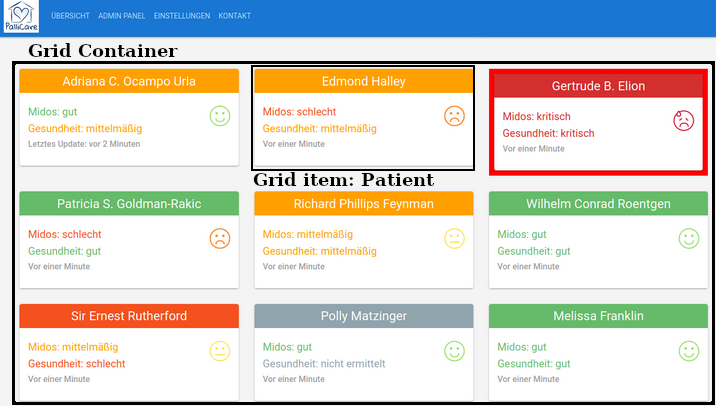
\includegraphics[width=6.17in,height=3.5in]{./media/image5.png}
  \end{center}
  \caption{Grid components}
  \label{fig:helptext2}
\end{figure} 

\textbf{Dock}

To see more details about one specific patient a dock\footnote{https://www.npmjs.com/package/react-dock} was implemented. On the click of a button it folds out and covers a large part of the screen. The dock can be closed with a button to the top left. Because the frontend was inspired by single page web-apps where one single source of information fuels all functionality this dock also uses the data of ‘patients’ context. It can be used to display graphs for example. A calendar will in the future allow a date range to be selected in which to view the patient data. \\

\begin{figure}[h]
	\centering
	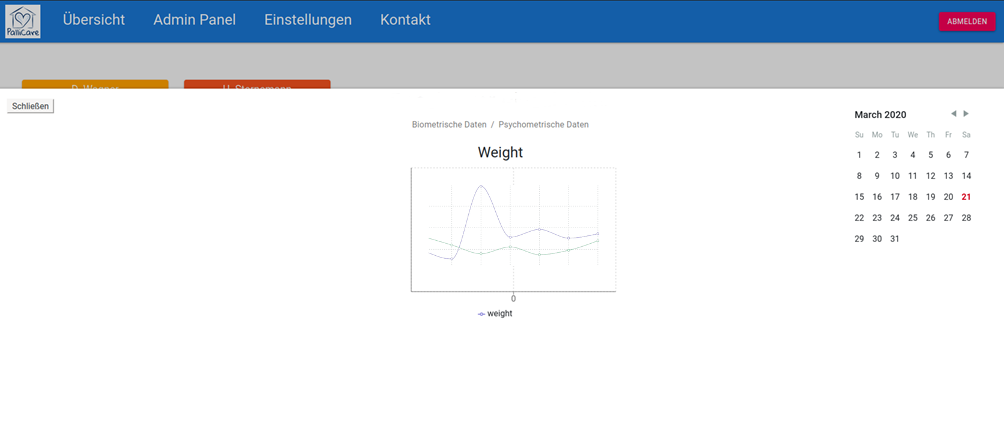
\includegraphics[width=6.69in,height=2.93in]{./media/image6.png}
	\caption{Expanded dock}
\end{figure}


\textbf{Security}

For realizing the auto logout feature of the web-app JWT, activity tracking\footnote{https://www.npmjs.com/package/react-idle-timer} and private routes\footnote{https://reacttraining.com/react-router} were leveraged. JWT tokens are getting obtained, refreshed and verified as soon as the user logs in and is active. Being active is determined by the user triggering mouse events like a button click or mouse movement. Should the user not be active for 10 minutes an auto logout will be performed and the JWT token will no longer be refreshed. This was done using a public route to the login screen and a private route that can only be accessed after user typed in the right credentials and if the JWT token is alive as well as if the user is active. To store the authentication status and perform the JWT verification for example a global context class like in PatientsContext.js was used in Authentication.js. 


\clearpage
\bibliographystyle{plainnat}
\bibliography{references}

\end{document}
%%% Local Variables: 
%%% mode: latex
%%% TeX-master: t
%%% End: 
